\RequirePackage[english=usenglishmax]{hyphsubst}
\documentclass[titlepage,letterpaper]{article}
\usepackage[utf8]{inputenc}
\usepackage[svgnames]{xcolor}
\usepackage{textcomp}
\usepackage{amsmath}
\usepackage[activate=true,final,tracking=true,kerning=true,spacing=true]{microtype}
\usepackage{graphicx}
\usepackage{changepage}
\usepackage{indentfirst}
\usepackage{caption}
\usepackage{pgf}
\usepackage{tikz}
\usepackage{comment}
\usepackage{subcaption}
\usepackage{pgfplots}
\pgfplotsset{compat=newest}
\usepackage{mathtools}
\usepackage{kantlipsum}
\usepackage[sorting=none, backend = biber]{biblatex}
\bibliography{references}
\usepackage{attachfile}
\usepackage{amsfonts}
\usepackage{amsmath}
\usepackage{placeins}
\usepackage{tcolorbox}
\usepackage{booktabs}
\setlength{\parindent}{4em}
\setlength{\parskip}{1em}
\usepackage{tabularx}
\usepackage{cleveref}
\usepackage[]{algorithm2e}
\setlength{\parindent}{3em}
\setlength{\parskip}{.75em}
%opening
\title{Sentiment Analysis in Text}
\author{Richard Lettich, Carmen Gaver, Bryce Taylor, Mary Grace Oster}
\date{Fall 2018}

\begin{document}

\maketitle

\begin{abstract}
This paper introduces an approach for how to predict sentiment from idioms and text using Long Short Term Memory (LSTM) Neural Networks. In general, the neural networks learn from loops and this allows the method to predict the correct sentiment with high success. Following an overview of LSTM Neural Networks, we show it's success rate on the Plutchik's Emotion data and the Twitter data. After illustrating its performance on on two data sets, a set of labeled data according to Plutchik's wheel of emotion and a sample of labeled Twitter data. We then show how it can be used on raw Twitter data. \\
\end{abstract}

\section{Introduction}

The goal of this project is to create a method which will accurately analyze a given text and predict the correct emotion which is expressed in the text. For many companies there is a high need for programs which can analyze a customer review and determine the appropriate underlying sentiment. Customer satisfaction plays a huge role in how companies compete. Novak, Sparl, and Azman explain how ``increased service quality positively influences customer satisfaction", which in turn leads to better financial results through increased customer loyalty \cite{BusinessCustomerSatisfaction}. Therefore companies need to know how well they are doing, how satisfied are the customers, where the company can improve, and much more. The goal of this project is to create a method which can accurately assign emotion to a given sentence.

It should be stated that Chick-fil-A is a customer service oriented brand. They desire to potentially use the methods described in this analysis as part of a larger project to discover how emotion relates to restaurant reviews in online comments and customer perception of service failure.

A spectrum of emotion (such as `satisfaction') would likely be best for this purpose. Since the goal is to determine what service failures and successes cause the strongest customer emotions and predict the former using the latter, it would be best to rank the emotion quantitatively. Determining that long wait times make people unhappy would provide no novel information, but being able to say that people become an order of magnitude more upset over one service failure than another would be beneficial as a tool of analysis. In addition, a spectrum of satisfaction would allow for better predictive capability when being used as a component of another analysis \cite{lowriwilliams}.

Secondly, it would be ideal to have a confidence value for the emotional prediction. If this sentiment analysis is used as part of another meta-tool, being able to provide an estimate of confidence would allow the meta-tool to weigh the sentiment analysis appropriately with its other variables.

Succinctly, we can define our desired result as follows: for a given snippet of text, give a numerical rating on a spectrum of a single (or possibly multiple) emotions along with an associated confidence score for this rating. To accomplish this goal, we use machine learning. 

\section{Machine Learning}

Machine Learning is the process of using a data set with known variables to create an algorithm which will predict a response variable \cite{Statlearning}. There are a variety of different machine learning methods, such as Quadratic Discriminant Analysis, Neural Networks, Ridge Regression, Logistic Regression, and much more \cite{Statlearning}. In this data set each sentence has an assigned emotion so the method will be a supervised learning method \cite{Statlearning}. Simply put a supervised learning method uses a data set which has both the predictor variable and the response variable to create an algorithm to predict the response variable \cite{Statlearning}. In this situation, the predictor variables are the sentences and the response variables are the emotions associated with each sentence \cite{Statlearning}. 

    The product of a supervised machine learning process is a model function which yield (a) predicted value(s) based on input data $x$. For the function to be built, prelabeled input data must be provided (i.e., pre produced sets of corresponding points, $(x,(f(x))$). While using $x$ and $f(x)$ oversimplifies the dimensionality of the input and outputs of the model, they will be continually used to explain machine learning conceptually.

In this paper, we utilize a supervising machine learning algorithm broadly categorized by the label of stochastic gradient descent\cite{stoch}. The process is not fundamentally different to regression.  There is an algorithm which attempts to find optimal parameters\cite{regression} \footnote{while the parameter of our model $f(x)$ is $x$, this is \emph{not} the parameter we are addressing} for the function f(x) to yield the best prediction. In the context of supervised machine learning, this algorithm is called the optimizer. For instance, if the optimizer was trying to produce a linear regression model, 
\[f(x) = mx + b \]
The optimizer’s goal would be to find the most ideal values of parameters $m$ and $b$. 

While this task is not daunting for such a simple function, it becomes much more complex for larger models that may contain thousands of parameters. However, at the simplest level, the process involves three parts: the model $f(x)$ itself, an optimization algorithm $\alpha$,  and a loss function $\lambda$.


\subsection{Loss function}

The loss function dignifies the error of the the predictions made by the model. It takes two parameters: the evaluation of our model at any given point($y_p$), and the actual value of the function at that given point, as provided by the input data set ($y_p$). A simple error function would be the distance from our prediction to what our actual value is
\[\lambda(y,y_p) =  |y - y_p| \]

The vast majority of loss functions are not so naive, but the moral this moral explanation holds.


\subsection{Optimizer function -- \textit{Stochastic gradient descent}}

In this paper, we use the \textit{Adam} optimizer, which is a tuned up version of stochastic gradient descent optimization. As it name alludes to, stochastic gradient descent optimizes the model function by descending the gradient of the loss function. 

Before explaining what that means, it should be known that SGD optimizers assumes  that if the loss function is smooth and continuous \textit{enough}, we are able to smooth it out, and the same rules of calculus still apply.

From this, if we take any point on the loss function, we are able to extrapolate that if we were modify our parameters \(p\) (where $p = [m, b,...]$), going in the direction opposite of the gradient of the loss function with respect those parameters ($\frac{\partial\lambda}{\partial p}$), we would be able to continuously re-evaluate and lower our error until we reach a gradient near zero, indicating we hypothetically found our optimal model parametrs

What does that mean? To illustrate simply, if we let $f(x)_{\text{act}}$ represent our actual data point, our loss function can be rewritten as 
\begin{align}
\lambda &=  |f(x)_{\text{act}} - f(x)| \nonumber\\
&= | f(x)_{\text{act}} -  (mx + b)\label{eq1}|
\end{align}
for any particular point $x$ in our data set, and its corresponding $f(x)_{\text{act}}$. If we were to modify  $m$  and graph it versus the error $\lambda$, we would see the resulting graph \cref{fig:m_vs_error}. 

SGD based optimizer functions find the gradient of this graph with respect to the optimization parameters (just $\frac{\partial\lambda}{\partial m}$ in this case). From this, they are able to accurately guess new parameters ($m$) in the direction of the gradient which will provide a lower error for our paticular test \(x\) and \(f(x)\) pair. 

This process is iterative, and the change in the parameter per iteration is called step size. Too large of a step size, and new parameter would `overshoot'. For instance if our $m$ was too small, `overshooting' would lead to it being too large.

\begin{figure}[h]
	\centering 
	\label{fig:m_vs_error}
	\caption{M vs. Error}
	
\includegraphics[scale=.11]{error_function.eps}
	\vspace{-55pt}
\end{figure}


\subsection{Caveats}
Of course, the model isn't as simple as linear regression. With hundreds of thousands to millions of possible data points, some are bound to disagree on how to adjust parameters. In addition, not all critical points where minima occur are absolute minima, possibly leading to the optimizer  getting `stuck' in a local minima. Sometimes optimizers have issues 'settling' in the lowest valley, often requiring lower learning rates.\cite{adaprop} Going in the direction opposite the gradient isn't rocket science. The differences between SGD optimizers mainly concern how work around these caveats while navigating the $\lambda$ graph \cite{adaprop,adam,rmsprop,moment}.

\section{Sentiment Analysis}
%Transition Needed$

In this project, ``sentiment analysis, also referred to as opinion mining, aims to automatically extract and classify sentiments, opinions, and emotions expressed in text" is performed on the Primary Emotion Data created by Lowri Williams \cite{lowriwilliams}. The purpose of Primary Emotion data set is to show the use-fullness of idioms in determining the emotion expressed in a given text. For example, an idiom might be ``we'd fight like cats and dogs"; from this sentence we can deduce that whomever is speaking would have awful fights with someone else \cite{lowriwilliams}. The labeled sentences were determined by contributors examined the sentences, rating their emotional content based on Plutchik's Wheel of Emotions and polarity categories (discussed in more detail below) \cite{lowriwilliams}. Sentiment classification problems often use polarity categories to represent and classify sentiment \cite{lowriwilliams}. Sentiment polarity can be positive, negative, and neutral. An example of sentiment polarity in the data is given by ``Mr.Jones was grinning from ear to ear"; that is a positive idiom; ``I was bored to tears at work today" is a negative statement. After deciding on the polarity it is very simple to then pick an emotion for the sentence \cite{lowriwilliams}. 

\section{Plutchik's Wheel of Emotion}

Plutchik's Wheel of Emotion, (\cref{plutchikemotionwheel}), has eight basic emotions including joy, trust, fear, surprise, sadness, disgust, anger, and anticipation. Each of the eight emotions has three levels of activation represented by color boldness. The emotion space is represented so that combinations of basic emotions derive secondary emotions. For example: joy+trust=love, anger+anticipation=aggression \cite{plutchik2001nature}.

The emotions on each leaf range in intensity. The emotions on the inner circle are the most intense and the emotions on the outer circle of each leaf are the least intense \cite{WheelofEmotion}. The emotions that fall between each leaf are a combination of each leaf's middle emotion \cite{WheelofEmotion}. For example, ``Trust + Fear = Submission". The Primary Emotion Data we use in this project has emotions from the middle of each leaf, the combinations emotions, and categories ``Neutral" and ``Ambiguous" \cite{lowriwilliams}.

\begin{figure}[ht]
	\center
	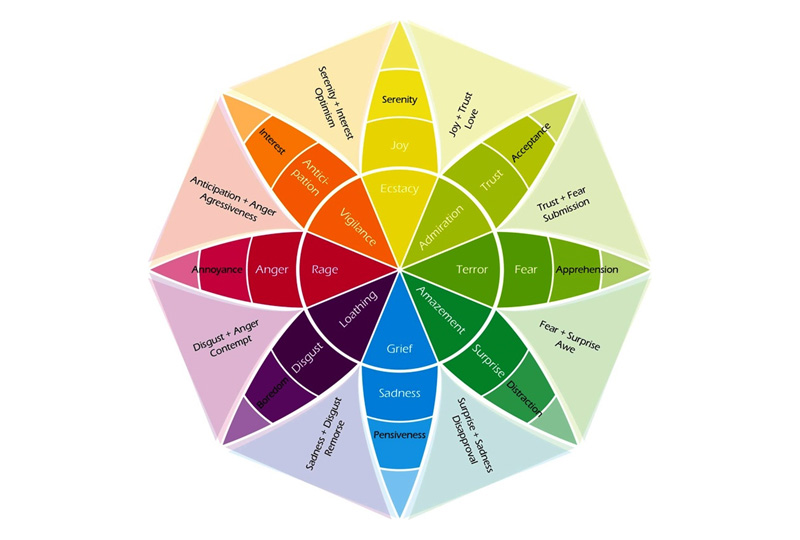
\includegraphics[width=4in]{PlutchikWheelOfEmotion.jpg}
	\caption{Plutchiks Wheel of Emotion \cite{WheelofEmotion}}
	\label{plutchikemotionwheel}
\end{figure}

\section{Primary Emotion Data}
Table \ref{PrimaryEmotionTable} gives a few examples of the sentences and labeled emotions in the data set which we will call the Primary Emotion data. The Primary Emotion data set contains around $2425$ emotion labeled sentences. For this project the data will be used to develop a model which, when given a text, will assign an emotion to the text. 
 
 \begin{center}
 	\captionof{table}{Primary Emotion Data}
 	\begin{tabular}{ |c|c| } 
 		\hline
 		Emotion & Sentence \\
 		\hline \hline
 		Neutral & Don't let him pick a fight now, we're almost home. \\
 		\hline
 		Optimism &  You must sink your differences. \\
 		\hline
 		Aggression & We'd fight like cat and dog.  \\ 
 		\hline
 		Disgust & For God's sake bury the hatchet. \\
 		\hline
 	\end{tabular}
 	\label{PrimaryEmotionTable}
 \end{center}

 
 Williams hypothesized that the use of idioms in sentiment analysis would increase the accuracy of predicting the correct emotion or category \cite{lowriwilliams}. Figure \ref{topsixgroups} shows a bar plot of the top six emotion groups, ranked by most frequently appearing groups in the data set. The emotion group ``Neutral" occurs the most, it comprises just over $20$ percent of the data set. 
 
% \begin{figure}[h!]
% 	\centering
% 	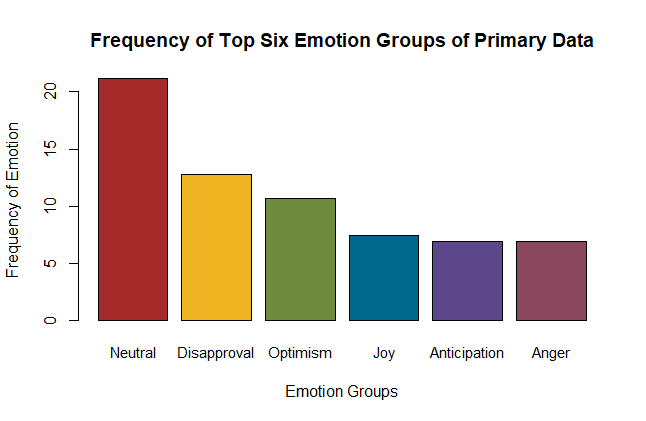
\includegraphics[width = 4.2in]{TopSixGroup1.png}
% 	\caption{Barplot of Frequency of Top Six Emotions in Primary Emotion Data}
% 	\label{TopSixGroup1}
% \end{figure}
 

 \begin{figure}[htb]
		\centering
 		\caption{Top Six Emotion Groups}
 		% Created by tikzDevice version 0.12 on 2018-12-07 16:26:20
% !TEX encoding = UTF-8 Unicode
\begin{tikzpicture}[x=1pt,y=1pt]
\definecolor{fillColor}{RGB}{255,255,255}
\path[use as bounding box,fill=fillColor,fill opacity=0.00] (0,0) rectangle (361.35,289.08);
\begin{scope}
\path[clip] (  0.00,  0.00) rectangle (361.35,289.08);
\definecolor{drawColor}{RGB}{0,0,0}
\definecolor{fillColor}{RGB}{165,42,42}

\path[draw=drawColor,line width= 0.4pt,line join=round,line cap=round,fill=fillColor] ( 59.83, 62.97) rectangle ( 97.78,239.88);
\definecolor{fillColor}{RGB}{238,180,34}

\path[draw=drawColor,line width= 0.4pt,line join=round,line cap=round,fill=fillColor] (105.38, 62.97) rectangle (143.33,169.98);
\definecolor{fillColor}{RGB}{110,139,61}

\path[draw=drawColor,line width= 0.4pt,line join=round,line cap=round,fill=fillColor] (150.92, 62.97) rectangle (188.88,152.09);
\definecolor{fillColor}{RGB}{0,104,139}

\path[draw=drawColor,line width= 0.4pt,line join=round,line cap=round,fill=fillColor] (196.47, 62.97) rectangle (234.43,124.92);
\definecolor{fillColor}{RGB}{93,71,139}

\path[draw=drawColor,line width= 0.4pt,line join=round,line cap=round,fill=fillColor] (242.02, 62.97) rectangle (279.97,120.95);
\definecolor{fillColor}{RGB}{139,71,93}

\path[draw=drawColor,line width= 0.4pt,line join=round,line cap=round,fill=fillColor] (287.57, 62.97) rectangle (325.52,120.95);
\end{scope}
\begin{scope}
\path[clip] (  0.00,  0.00) rectangle (361.35,289.08);
\definecolor{drawColor}{RGB}{0,0,0}

\node[text=drawColor,anchor=base,inner sep=0pt, outer sep=0pt, scale=  0.80] at ( 78.81, 39.60) {Neutral};

\node[text=drawColor,anchor=base,inner sep=0pt, outer sep=0pt, scale=  0.80] at (124.35, 39.60) {Disapproval};

\node[text=drawColor,anchor=base,inner sep=0pt, outer sep=0pt, scale=  0.80] at (169.90, 39.60) {Optimism};

\node[text=drawColor,anchor=base,inner sep=0pt, outer sep=0pt, scale=  0.80] at (215.45, 39.60) {Joy};

\node[text=drawColor,anchor=base,inner sep=0pt, outer sep=0pt, scale=  0.80] at (261.00, 39.60) {Anticipation};

\node[text=drawColor,anchor=base,inner sep=0pt, outer sep=0pt, scale=  0.80] at (306.54, 39.60) {Anger};
\end{scope}
\begin{scope}
\path[clip] (  0.00,  0.00) rectangle (361.35,289.08);
\definecolor{drawColor}{RGB}{0,0,0}

\node[text=drawColor,anchor=base west,inner sep=0pt, outer sep=0pt, scale=  1.20] at ( 100.00,275.61) {\bfseries Top Six Emotion Groups};

\node[text=drawColor,anchor=base,inner sep=0pt, outer sep=0pt, scale=  1.00] at (192.68, 15.60) {Emotion Groups};

\node[text=drawColor,rotate= 90.00,anchor=base,inner sep=0pt, outer sep=0pt, scale=  1.00] at ( 10.80,150.54) {Frequency of Emotion};
\end{scope}
\begin{scope}
\path[clip] (  0.00,  0.00) rectangle (361.35,289.08);
\definecolor{drawColor}{RGB}{0,0,0}

\path[draw=drawColor,line width= 0.4pt,line join=round,line cap=round] ( 49.20, 62.97) -- ( 49.20,230.21);

\path[draw=drawColor,line width= 0.4pt,line join=round,line cap=round] ( 49.20, 62.97) -- ( 43.20, 62.97);

\path[draw=drawColor,line width= 0.4pt,line join=round,line cap=round] ( 49.20,104.78) -- ( 43.20,104.78);

\path[draw=drawColor,line width= 0.4pt,line join=round,line cap=round] ( 49.20,146.59) -- ( 43.20,146.59);

\path[draw=drawColor,line width= 0.4pt,line join=round,line cap=round] ( 49.20,188.40) -- ( 43.20,188.40);

\path[draw=drawColor,line width= 0.4pt,line join=round,line cap=round] ( 49.20,230.21) -- ( 43.20,230.21);

\node[text=drawColor,rotate= 90.00,anchor=base,inner sep=0pt, outer sep=0pt, scale=  1.00] at ( 34.80, 62.97) {0};

\node[text=drawColor,rotate= 90.00,anchor=base,inner sep=0pt, outer sep=0pt, scale=  1.00] at ( 34.80,104.78) {5};

\node[text=drawColor,rotate= 90.00,anchor=base,inner sep=0pt, outer sep=0pt, scale=  1.00] at ( 34.80,146.59) {10};

\node[text=drawColor,rotate= 90.00,anchor=base,inner sep=0pt, outer sep=0pt, scale=  1.00] at ( 34.80,188.40) {15};

\node[text=drawColor,rotate= 90.00,anchor=base,inner sep=0pt, outer sep=0pt, scale=  1.00] at ( 34.80,230.21) {20};
\end{scope}
\end{tikzpicture}

 		\label{topsixgroups}
 \end{figure}
 	
 %\clearpage
 
\section{Methods}

\subsection{Text Mining}
The goal of this project is to implement a method which when given a bit of text will sort the text into one of the emotions categories. The first step in this project is to do some basic text mining. Text mining is the process of ``cleaning" a data set most raw data will contain punctuation, capitalizations, quotes, tenses, and much more \cite{TextMining}. For most text analysis, not all words are needed. Words like ``the", ``a", ``an", and others, known as ``stopwords", are not important to build a model which will assign emotion or predict a star rating \cite{TextMining}. 

Once the data is clean, each sentence must be broken down into ``tokens". A token can be each sentence, each word, or even a set of words \cite{TextMining}. For this project each token represents a word in each sentence. 

\subsection{Term Frequency Matrix}
The next step in the project is to create a term frequency matrix. Specifically, the term frequency matrix is a matrix with columns corresponding to the emotions we want to detect, and rows representing each word; the matrix itself will contain the number of times a word appears in the assigned emotion category. Since the data set contains over six thousand words, the frequency matrix will be large.

\subsection{Adam Optimizer}
The Adam optimizer is the de facto successor to a RMSProp \cite{adam}. In RMSProp initial values must be chosen for some variables in the optimization algorithm \cite{adam}. This can lead to bias. The Adam optimizer improves upon RMSProp by correcting this bias in later calculations. In addition, while RMSProp calculates its effective step size using momentum, Adam implements a `Signal to Noise' method, changing it based on a smooth gradient moving average (moment estimation, $m_t$) and a moving variance estimation ($v_t$). This means the rate at which it navigates the gradient is a metaphorical function of confidence: the less steady the gradient, the slower it goes. The Adam optimizer has proved to produce consistently excellent results, therefore it was chosen as the benchmark optimizer for this project.

Algorithm $1$ gives a pseudo-code representation of the Adam optimizer (Algorithm $1$). Refer to Table \ref{adam_table} for an explanation of the components and notation in the description of the optimizer.

\begin{table}[]
	\begin{adjustwidth}{-1in}{-1in}
		\centering
		\SetAlgoLined
		\caption{Glossary of notation used in Adam optimizer}
		\label{adam_table}
		\begin{tabular}{lll}
			\hline
			& \textbf{Description}                                                   & \textbf{Elaboration}                                                                                                                                                                                                                                               \\ \hline
			\multicolumn{1}{|l}{$f(x)$}    & Objective function                                                     & \multicolumn{1}{l|}{\begin{tabular}[c]{@{}l@{}}The term to be minimized. This is not the model function.\\ If $g(x)$ function we wish to optimize, and $\lambda$ is\\ our loss function, $f(x) = \lambda \circ g(x)$. See eq. 1 \\ for clarification\end{tabular}} \\ \hline
			\multicolumn{1}{|l}{$\alpha$}  & Step Size                                                              & \multicolumn{1}{l|}{Size of increment of change of parameters per $t$.}                                                                                                                                                                                            \\ \hline
			\multicolumn{1}{|l}{$t$}       & Time                                                                   & \multicolumn{1}{l|}{\begin{tabular}[c]{@{}l@{}}Integer value to keep track of iteration of optimizer.\\ Pragmatically, the iterator variable of the optimizer for loop.\end{tabular}}                                                                              \\ \hline
			\multicolumn{1}{|l}{$\odot$}   & Component-Wise Multiplication                                          & \multicolumn{1}{l|}{\begin{tabular}[c]{@{}l@{}}$[a,b,c, ..] \odot [d, e,f,...] = [ad,be,cf,...]$, When a non\\ scalar $n$ value is raised to a power $p$, it implies\\  $n \odot n^{p-1}$\end{tabular}}                                                                      \\ \hline
			\multicolumn{1}{|l}{$m_t$}     & Moment  Estimation                                                     & \multicolumn{1}{l|}{\begin{tabular}[c]{@{}l@{}}Moving average of gradient -- a smoothed version of\\ the gradient function. Defined by first moment of \\ gradient.\end{tabular}}                                                                                  \\ \hline
			\multicolumn{1}{|l}{$v_t$}     & Variance Estimation                                                    & \multicolumn{1}{l|}{\begin{tabular}[c]{@{}l@{}}Variance of gradient function as defined by second\\  moment of gradient.\end{tabular}}                                                                                                                             \\ \hline
			\multicolumn{1}{|l}{$\theta$}  & \begin{tabular}[c]{@{}l@{}}Parameters of Model\\ Function\end{tabular} & \multicolumn{1}{l|}{Parameters of model. Earlier denoted $p$ and $m$.}                                                                                                                                                                                             \\ \hline
			\multicolumn{1}{|l}{$g_t$}     & Gradient                                                               & \multicolumn{1}{l|}{\begin{tabular}[c]{@{}l@{}}Gradient with respect to optimization parameters. \\ Earlier denoted  $\frac{\partial \lambda}{\partial p}$, more appropriately denoted $\nabla_\theta f(\theta)$\end{tabular}}                                   \\ \hline
			\multicolumn{1}{|l}{$\beta_1$} & Decay rate of $m_t$                                                    & \multicolumn{1}{l|}{\begin{tabular}[c]{@{}l@{}}Multiplied by previous $m_t$ each iteration($t$)  \\ before adding new information. \\ \\ Acceptable range [0,1), Default .9\end{tabular}}                                                                           \\ \hline
			\multicolumn{1}{|l}{$\beta_2$} & Decay rate of $v_t$                                                    & \multicolumn{1}{l|}{\begin{tabular}[c]{@{}l@{}}Multiplied by previous $v_t$ each iteration($t$) \\ before taking into account  \\ \\ Acceptable range: [0,1), Default .999\end{tabular}}                                                                           \\ \hline
		\end{tabular}
	\end{adjustwidth}
\end{table}

\newcommand{\assn}{\mathrel{{:}{=}}}
\begin{algorithm}[]
	\caption{Pseudo-code representation of Adam optimizer. The $\mathrel{{:}{=}}$ ligature  represents assignment.}
	\label{adam_alg}
	\KwData{$\theta_0$, $f(x)$ (initial function parameters, unoptimized objective function), }
	\textbf{Initialize variables}:
	$\{m_0,V_0,t\} = 0$\;
	\vspace{3.5mm}
	\While{\text{model is not fitted}}{
		\begin{align*}
		t &\assn t +  1\\ 
		g_t &\assn \nabla_\theta f\left(\theta_{t-1}\right)\;  \hspace{2mm} \text{Find actual gradient. }\\
		m_t &\assn \beta_1 m_{t-1} + (1-\beta_1)g_t\\
		&\text{Assign new gradient moving average, where previous} \\
		&\text{gradients have weight} \frac{\beta_1}{1} \\
		v_t &\assn \beta_2 m_{t-1} + (1-\beta_1)g_t^2 \\
		&\text{Assign a new moving variance estimation in the same manner,}\\
		&\text{but instead using } \beta_2\\
		\widehat{m_t} &\assn \frac{m_t}{1-\beta_1^t}\\
		\widehat{v_t} &\assn \frac{v_t}{1-\beta_2^t}\\
		&\text{Bias results from where we initiated } v_t \text{ with zero. The last two}\\
		&\text{statements correct that bias. See Adam paper.}\\
		\theta_t &\assn \theta_{t-1} - \alpha\frac{ \widehat{m_t}}{\sqrt{v_t} + \epsilon}\\
		& \text{Update the parameters going in the opposite direction of our new}\\
		& \text{calculated gradient average. Weigh update by dividing by } \sqrt{\widehat{v_t}}, \\
		& \text{(more noise, lower effective step size.)}
		\end{align*}
	}
	\vspace{3.5mm}
\end{algorithm}
%% Perhaps move this gradient paragraph to the Loss Function Section %%

\paragraph{Gradient} - The gradient of a function $\nabla_\theta f(\theta)$ evaluated at point $\theta$ is by definition the direction of steepest ascent at point $\theta$. We use this, as we are trying to reduce our inaccuracy/loss by moving in the direction of steepest \textit{descent} \mbox{(i.e. $-\nabla_\theta f(\theta)$)}. 

\paragraph{Gradient Moving Average}

The Adam optimizer does not just naively use the gradient itself, but instead smooths it using the exponential moving average as originally described by J. Stuart Hunter\cite{EMA}. This formula gives a much less noisy curve to descend, and helps prevent the optimizer from plateauing in local minima. Although used recursively here, a non recursive equivalent is given by
\[m_t = \sum_{t=0}^{t_f} \left(1-\beta_1\right) \beta_1^{t_f-t}\nabla_\theta f\left(\theta_{t}\right)^2.\]
()Although purely semantic, in the original EMA formula, \(\beta_1\) and \(\left(1-\beta_1\right)\) are switched).


\paragraph{Moving Variance}
The moving variance is used to modulate the learning rate of the function, depending on how noisy the slope is. For an intuitive sense, recall that standard deviation is given by:
\[\sigma = \sqrt{\sum \left(x_n - \bar{x}\right)}.\]
If we replace \(x_n\) with \ \(\nabla_\theta f(\theta)\), and \(\bar{x}\) with a gradient of \(\vec{0}\), we get \footnote{\(f\left(\theta_{t}\right)^2 \implies \) component wise multiplication}
\[\sigma = \sqrt{\sum \left(\nabla_\theta f(\theta)\right)^2}.\]
Applying the same exponential moving average to this `variance from the zero gradient' yields a moving average in the same manner of the moving average of the gradient. Albeit, the variance is more conservative, as \(\beta_2\) is typically larger than \(\beta_1\).

\subsection{Model Layers}

A different approach was used for each model. Historically, Bidirectional LSTM has shown better results for textual analysis \cite{Keras.io}. However, in testing, it performed equivalently or worse than regular LSTM, and significantly increased time to convergence. However, implementing Bi-directional LSTM on the idiom data has yielded a significant boost, raising accuracy approximately 5\% over regular LSTM.

\subsection{Dropout Technique}
Dropout is a regularization technique for the Long Short Term Memory Neural Networks. It is a new approach that randomly picks neurons to be dropped from the training network \cite{NeuralNet}. Those neurons are completely neglected. The goal of using this approach is to keep the neural network from overfitting to the training set. The dropout rate that is used and experimented with is between 20-50\% \cite{NeuralNet}.
Dropout is a regularization technique for the Long Short Term Memory Neural Networks. It is a new approach that randomly picks neurons to be dropped from the training network \cite{NeuralNet}. Those neurons are completely neglected. The goal of using this approach is to keep the neural network from over-fitting to the training set. The dropout rate that is used and experimented with is between 20-50\% \cite{NeuralNet}.

\subsection{Validation Accuracy}
Figure \ref{valepoch} shows the change in validation accuracy by epoch, which is the number of times the model has seen the training data set, for a few different methods. We used both mono-directional and bi-directional neural nets with up to three hidden layers. As we can see each method starts at approximately the same level of validation accuracy. The bidirectional method with two hidden layers appears to have the most consistent accuracy over the epochs; it levels off after five epochs without much fluctuation in validation accuracy. 

\begin{figure}[htb]
	\centering
	\resizebox{4in}{!}{% Created by tikzDevice version 0.12 on 2018-12-03 20:41:36
% !TEX encoding = UTF-8 Unicode
\begin{tikzpicture}[x=1pt,y=1pt]
\definecolor{fillColor}{RGB}{255,255,255}
\path[use as bounding box,fill=fillColor,fill opacity=0.00] (0,0) rectangle (361.35,361.35);
\begin{scope}
\path[clip] ( 49.20, 61.20) rectangle (336.15,312.15);
\definecolor{drawColor}{RGB}{255,255,255}

\path[draw=drawColor,line width= 0.8pt,line join=round,line cap=round] ( 59.83, 70.49) circle (  2.25);

\path[draw=drawColor,line width= 0.8pt,line join=round,line cap=round] ( 73.81,168.50) circle (  2.25);

\path[draw=drawColor,line width= 0.8pt,line join=round,line cap=round] ( 87.80,247.53) circle (  2.25);

\path[draw=drawColor,line width= 0.8pt,line join=round,line cap=round] (101.78,253.85) circle (  2.25);

\path[draw=drawColor,line width= 0.8pt,line join=round,line cap=round] (115.76,266.50) circle (  2.25);

\path[draw=drawColor,line width= 0.8pt,line join=round,line cap=round] (129.75,274.40) circle (  2.25);

\path[draw=drawColor,line width= 0.8pt,line join=round,line cap=round] (143.73,283.89) circle (  2.25);

\path[draw=drawColor,line width= 0.8pt,line join=round,line cap=round] (157.72,290.21) circle (  2.25);

\path[draw=drawColor,line width= 0.8pt,line join=round,line cap=round] (171.70,296.53) circle (  2.25);

\path[draw=drawColor,line width= 0.8pt,line join=round,line cap=round] (185.68,294.95) circle (  2.25);

\path[draw=drawColor,line width= 0.8pt,line join=round,line cap=round] (199.67,301.27) circle (  2.25);

\path[draw=drawColor,line width= 0.8pt,line join=round,line cap=round] (213.65,298.11) circle (  2.25);

\path[draw=drawColor,line width= 0.8pt,line join=round,line cap=round] (227.63,299.69) circle (  2.25);

\path[draw=drawColor,line width= 0.8pt,line join=round,line cap=round] (241.62,302.86) circle (  2.25);

\path[draw=drawColor,line width= 0.8pt,line join=round,line cap=round] (255.60,299.69) circle (  2.25);

\path[draw=drawColor,line width= 0.8pt,line join=round,line cap=round] (269.59,302.86) circle (  2.25);

\path[draw=drawColor,line width= 0.8pt,line join=round,line cap=round] (283.57,293.37) circle (  2.25);

\path[draw=drawColor,line width= 0.8pt,line join=round,line cap=round] (297.55,296.53) circle (  2.25);

\path[draw=drawColor,line width= 0.8pt,line join=round,line cap=round] (311.54,299.69) circle (  2.25);

\path[draw=drawColor,line width= 0.8pt,line join=round,line cap=round] (325.52,288.63) circle (  2.25);
\end{scope}
\begin{scope}
\path[clip] (  0.00,  0.00) rectangle (361.35,361.35);
\definecolor{drawColor}{RGB}{0,0,0}

\path[draw=drawColor,line width= 0.4pt,line join=round,line cap=round] ( 59.83, 61.20) -- (269.59, 61.20);

\path[draw=drawColor,line width= 0.4pt,line join=round,line cap=round] ( 59.83, 61.20) -- ( 59.83, 55.20);

\path[draw=drawColor,line width= 0.4pt,line join=round,line cap=round] (129.75, 61.20) -- (129.75, 55.20);

\path[draw=drawColor,line width= 0.4pt,line join=round,line cap=round] (199.67, 61.20) -- (199.67, 55.20);

\path[draw=drawColor,line width= 0.4pt,line join=round,line cap=round] (269.59, 61.20) -- (269.59, 55.20);

\node[text=drawColor,anchor=base,inner sep=0pt, outer sep=0pt, scale=  1.00] at ( 59.83, 39.60) {0};

\node[text=drawColor,anchor=base,inner sep=0pt, outer sep=0pt, scale=  1.00] at (129.75, 39.60) {5};

\node[text=drawColor,anchor=base,inner sep=0pt, outer sep=0pt, scale=  1.00] at (199.67, 39.60) {10};

\node[text=drawColor,anchor=base,inner sep=0pt, outer sep=0pt, scale=  1.00] at (269.59, 39.60) {15};

\path[draw=drawColor,line width= 0.4pt,line join=round,line cap=round] ( 49.20, 83.08) -- ( 49.20,279.59);

\path[draw=drawColor,line width= 0.4pt,line join=round,line cap=round] ( 49.20, 83.08) -- ( 43.20, 83.08);

\path[draw=drawColor,line width= 0.4pt,line join=round,line cap=round] ( 49.20,132.20) -- ( 43.20,132.20);

\path[draw=drawColor,line width= 0.4pt,line join=round,line cap=round] ( 49.20,181.33) -- ( 43.20,181.33);

\path[draw=drawColor,line width= 0.4pt,line join=round,line cap=round] ( 49.20,230.46) -- ( 43.20,230.46);

\path[draw=drawColor,line width= 0.4pt,line join=round,line cap=round] ( 49.20,279.59) -- ( 43.20,279.59);

\node[text=drawColor,rotate= 90.00,anchor=base,inner sep=0pt, outer sep=0pt, scale=  1.00] at ( 34.80, 83.08) {0.74};

\node[text=drawColor,rotate= 90.00,anchor=base,inner sep=0pt, outer sep=0pt, scale=  1.00] at ( 34.80,132.20) {0.76};

\node[text=drawColor,rotate= 90.00,anchor=base,inner sep=0pt, outer sep=0pt, scale=  1.00] at ( 34.80,181.33) {0.78};

\node[text=drawColor,rotate= 90.00,anchor=base,inner sep=0pt, outer sep=0pt, scale=  1.00] at ( 34.80,230.46) {0.80};

\node[text=drawColor,rotate= 90.00,anchor=base,inner sep=0pt, outer sep=0pt, scale=  1.00] at ( 34.80,279.59) {0.82};

\path[draw=drawColor,line width= 0.4pt,line join=round,line cap=round] ( 49.20, 61.20) --
	(336.15, 61.20) --
	(336.15,312.15) --
	( 49.20,312.15) --
	( 49.20, 61.20);
\end{scope}
\begin{scope}
\path[clip] (  0.00,  0.00) rectangle (361.35,361.35);
\definecolor{drawColor}{RGB}{0,0,0}

\node[text=drawColor,anchor=base,inner sep=0pt, outer sep=0pt, scale=  1.20] at (192.68,332.61) {\bfseries Validation Accuracy by Epoch};

\node[text=drawColor,anchor=base,inner sep=0pt, outer sep=0pt, scale=  1.00] at (192.68, 15.60) {Epoch};

\node[text=drawColor,rotate= 90.00,anchor=base,inner sep=0pt, outer sep=0pt, scale=  1.00] at ( 10.80,186.68) {Validation Accuracy};
\end{scope}
\begin{scope}
\path[clip] ( 49.20, 61.20) rectangle (336.15,312.15);
\definecolor{drawColor}{RGB}{104,34,139}

\path[draw=drawColor,line width= 0.8pt,line join=round,line cap=round] ( 59.83, 70.49) --
	( 73.81,168.50) --
	( 87.80,247.53) --
	(101.78,253.85) --
	(115.76,266.50) --
	(129.75,274.40) --
	(143.73,283.89) --
	(157.72,290.21) --
	(171.70,296.53) --
	(185.68,294.95) --
	(199.67,301.27) --
	(213.65,298.11) --
	(227.63,299.69) --
	(241.62,302.86) --
	(255.60,299.69) --
	(269.59,302.86) --
	(283.57,293.37) --
	(297.55,296.53) --
	(311.54,299.69) --
	(325.52,288.63);
\definecolor{drawColor}{RGB}{110,139,61}

\path[draw=drawColor,line width= 0.8pt,line join=round,line cap=round] ( 63.62,  0.00) --
	( 73.81,159.01) --
	( 87.80,226.98) --
	(101.78,241.21) --
	(115.76,266.50) --
	(129.75,271.24) --
	(143.73,261.76) --
	(157.72,269.66) --
	(171.70,280.73) --
	(185.68,293.37) --
	(199.67,287.05) --
	(213.65,283.89) --
	(227.63,287.05) --
	(241.62,288.63) --
	(255.60,304.44) --
	(269.59,283.89) --
	(283.57,298.11) --
	(297.55,293.37) --
	(311.54,280.73) --
	(325.52,285.47);
\definecolor{drawColor}{RGB}{139,26,26}

\path[draw=drawColor,line width= 0.8pt,line join=round,line cap=round] ( 67.02,  0.00) --
	( 73.81,130.56) --
	( 87.80,214.34) --
	(101.78,250.69) --
	(115.76,250.69) --
	(129.75,280.73) --
	(143.73,290.21) --
	(157.72,291.79) --
	(171.70,291.79) --
	(185.68,291.79) --
	(199.67,302.86) --
	(213.65,298.11) --
	(227.63,296.53) --
	(241.62,298.11) --
	(255.60,291.79) --
	(269.59,293.37) --
	(283.57,294.95) --
	(297.55,302.86) --
	(311.54,282.31) --
	(325.52,296.53);
\definecolor{drawColor}{RGB}{83,134,139}

\path[draw=drawColor,line width= 0.8pt,line join=round,line cap=round] ( 59.83, 57.85) --
	( 73.81,130.56) --
	( 87.80,214.34) --
	(101.78,223.82) --
	(115.76,258.60) --
	(129.75,277.56) --
	(143.73,266.50) --
	(157.72,291.79) --
	(171.70,301.27) --
	(185.68,282.31) --
	(199.67,275.98) --
	(213.65,306.02) --
	(227.63,299.69) --
	(241.62,294.95) --
	(255.60,291.79) --
	(269.59,298.11) --
	(283.57,280.73) --
	(297.55,294.95) --
	(311.54,290.21) --
	(325.52,287.05);
\definecolor{drawColor}{RGB}{0,0,0}

\path[draw=drawColor,line width= 0.4pt,line join=round,line cap=round] (171.70,181.33) rectangle (286.46,121.33);
\definecolor{drawColor}{RGB}{104,34,139}

\path[draw=drawColor,line width= 0.4pt,dash pattern=on 1pt off 3pt ,line join=round,line cap=round] (174.40,169.33) -- (192.40,169.33);
\definecolor{drawColor}{RGB}{110,139,61}

\path[draw=drawColor,line width= 0.4pt,dash pattern=on 1pt off 3pt ,line join=round,line cap=round] (174.40,157.33) -- (192.40,157.33);
\definecolor{drawColor}{RGB}{139,26,26}

\path[draw=drawColor,line width= 0.4pt,dash pattern=on 1pt off 3pt ,line join=round,line cap=round] (174.40,145.33) -- (192.40,145.33);
\definecolor{drawColor}{RGB}{83,134,139}

\path[draw=drawColor,line width= 0.4pt,dash pattern=on 1pt off 3pt ,line join=round,line cap=round] (174.40,133.33) -- (192.40,133.33);
\definecolor{drawColor}{RGB}{104,34,139}

\path[draw=drawColor,line width= 0.4pt,line join=round,line cap=round] (183.40,169.33) circle (  2.25);
\definecolor{drawColor}{RGB}{110,139,61}

\path[draw=drawColor,line width= 0.4pt,line join=round,line cap=round] (183.40,157.33) circle (  2.25);
\definecolor{drawColor}{RGB}{139,26,26}

\path[draw=drawColor,line width= 0.4pt,line join=round,line cap=round] (183.40,145.33) circle (  2.25);
\definecolor{drawColor}{RGB}{83,134,139}

\path[draw=drawColor,line width= 0.4pt,line join=round,line cap=round] (183.40,133.33) circle (  2.25);
\definecolor{drawColor}{RGB}{0,0,0}

\node[text=drawColor,anchor=base west,inner sep=0pt, outer sep=0pt, scale=  1.00] at (201.40,165.89) {Bidirectional 2};

\node[text=drawColor,anchor=base west,inner sep=0pt, outer sep=0pt, scale=  1.00] at (201.40,153.89) {Singledirectional 1};

\node[text=drawColor,anchor=base west,inner sep=0pt, outer sep=0pt, scale=  1.00] at (201.40,141.89) {Bidirectional 3};

\node[text=drawColor,anchor=base west,inner sep=0pt, outer sep=0pt, scale=  1.00] at (201.40,129.89) {Bidirectional 1};
\end{scope}
\end{tikzpicture}
}
	\caption{Validation Accuracy by Epoch}\label{valepoch}
\end{figure}
\section{Positive and Negative Groups}

For this project, we first ran our method on Primary Emotion Data \cite{lowriwilliams}, then we ran it on a sample of labeled Twitter data \cite{LabeledTwitter} data to determine if the method would work on both sets of data and accurately predict the underlying emotion of a text. In both cases the data was broken into two groups, positive and negative. Once the data was labeled as positive and negative, the data was then split into a training set and a testing or validation set. Next the data goes through the LSTM method which is programmed to go through each element of the data set and learn the appropriate response variable. In this project the LSTM network loops through each sentence and the corresponding emotion category and then continues through each sentence. This LSTM network learns the proportion of each emotion category. Once the LSTM network has gone through the entire training data set, it will predict emotion in the test data set. The method will predict the same proportion of emotion categories from the test set as are represented in the training data set. 

\section{Results}

\subsection{Primary Emotion Data Results}
The Primary Emotion Data positive group contained the categories joy, love, optimism, trust, and awe; in the negative group we have anger, disgust, sadness, aggression, contempt, disapproval, and remorse. The rest of the emotion groups are disregarded since they do not fall into either positive or negative categorizations.

The results using this model on the training set, which was made up of $80$ percent of the data, was an accuracy of around $89$ percent. The testing set was composed of the remaining $20$ percent of the data and had an accuracy of $74$ percent. The gap in the training and testing accuracy suggests that the method is over-fitting to  the training set. Put more simply, the method is learning the patterns in the training data set rather than learning the overall dynamics of the data. Consequently the method can accurately predict the training set, but it makes less accurate predictions for data it has not yet seen.

Figure \ref{primemresult} shows a barplot of both positive predictions and negative predictions for the Primary Emotion Data testing set. The light blue shows the percent of correct predictions for both categories. The dark blue bar indicates the percent of False Negatives, or sentences which should have been classified as positive for the positive bar, or negative in the negative bar. For the Primary Emotion data the model is most accurately predicting the positive emotions; meanwhile it isn't doing quiet as well with the negative emotion group. We would prefer more accuracy in the prediction of negative sentiment. 

% add a transition here%

Companies want to know which areas they need to improve. A big part of that process is finding out where the company is going wrong with the customer. This information is found in reviews from the customer, whether through some social media website, Yelp!, or reviews posted directly to the company. At some point the company is going to see the comment, tweet, or review and have to analyze it. However a problem with this is the volume of reviews a company, especially a big chain restaurant will receive. A model like the one developed in this project could go through a large set of reviews and tell the company which reviews should be examined more closely, or which reviews are the most important. In other words, the model used in this project could potentially tell a company which reviews are the most negative and should be investigated further.   

%\begin{figure}[h!]
%	\center
%	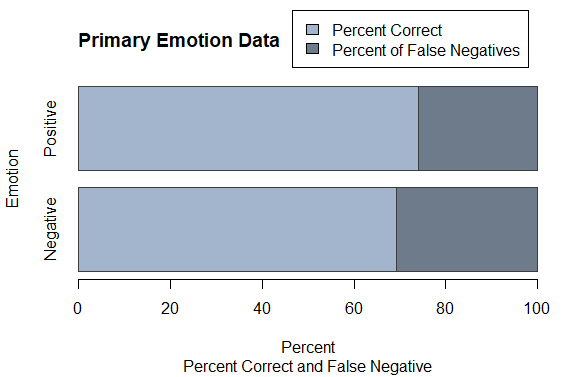
\includegraphics[width = 3.5in]{BarPlotPrimaryResults.png}
%	\caption{Barplot of Results of Primary Emotion Data, Positive and Negative Categories}
%	\label{bpprimem}
%\end{figure}

%\begin{subfigure}[]{6cm} \centering \resizebox{\linewidth}{!}{% This file was created by matplotlib2tikz v0.6.18.
\begin{tikzpicture}

\begin{axis}[
axis background/.style={fill=white!89.80392156862746!black},
axis line style={white},
height=6cm,
tick align=outside,
tick pos=left,
title={Sentiment Distribution of Chick-fil-A Twitter Comments},
width=9cm,
x grid style={white},
xlabel={Positive Sentiment Score},
xmajorgrids,
xmin=0, xmax=1,
xtick={0,0.2,0.4,0.6,0.8,1},
xticklabels={0.0,0.2,0.4,0.6,0.8,1.0},
y grid style={white},
ylabel={Percent of Scored Comments},
ymajorgrids,
ymin=0, ymax=7
]
\draw[fill=red,draw opacity=0] (axis cs:0.0219790190458298,0) rectangle (axis cs:0.0463351532816887,0.948521150382389);
\draw[fill=red,draw opacity=0] (axis cs:0.0463351532816887,0) rectangle (axis cs:0.0706912875175476,1.49053335030431);
\draw[fill=red,draw opacity=0] (axis cs:0.0706912875175476,0) rectangle (axis cs:0.0950474217534065,0.813018191075078);
\draw[fill=red,draw opacity=0] (axis cs:0.0950474292039871,0) rectangle (axis cs:0.119403563439846,0.677515159229232);
\draw[fill=red,draw opacity=0] (axis cs:0.119403563439846,0) rectangle (axis cs:0.143759697675705,1.62603588474317);
\draw[fill=red,draw opacity=0] (axis cs:0.143759697675705,0) rectangle (axis cs:0.168115824460983,0.271006146592908);
\draw[fill=red,draw opacity=0] (axis cs:0.168115824460983,0) rectangle (axis cs:0.192471966147423,1.21952691355738);
\draw[fill=red,draw opacity=0] (axis cs:0.192471966147423,0) rectangle (axis cs:0.216828092932701,0.813018439778725);
\draw[fill=red,draw opacity=0] (axis cs:0.216828107833862,0) rectangle (axis cs:0.241184249520302,0.813017942371583);
\draw[fill=red,draw opacity=0] (axis cs:0.241184234619141,0) rectangle (axis cs:0.265540361404419,0.94852151307518);
\draw[fill=red,draw opacity=0] (axis cs:0.265540361404419,0) rectangle (axis cs:0.289896488189697,0.813018439778725);
\draw[fill=red,draw opacity=0] (axis cs:0.289896488189697,0) rectangle (axis cs:0.314252644777298,1.35502907494175);
\draw[fill=red,draw opacity=0] (axis cs:0.314252644777298,0) rectangle (axis cs:0.338608771562576,0.271006146592908);
\draw[fill=red,draw opacity=0] (axis cs:0.338608771562576,0) rectangle (axis cs:0.362964898347855,0.542012293185817);
\draw[fill=red,draw opacity=0] (axis cs:0.362964898347855,0) rectangle (axis cs:0.387321025133133,0.813018439778725);
\draw[fill=red,draw opacity=0] (axis cs:0.387321054935455,0) rectangle (axis cs:0.411677211523056,0.27100581498835);
\draw[fill=red,draw opacity=0] (axis cs:0.411677181720734,0) rectangle (axis cs:0.436033308506012,1.08402458637163);
\draw[fill=red,draw opacity=0] (axis cs:0.436033308506012,0) rectangle (axis cs:0.46038943529129,0.542012293185817);
\draw[fill=red,draw opacity=0] (axis cs:0.46038943529129,0) rectangle (axis cs:0.484745562076569,0.406509219889363);
\draw[fill=red,draw opacity=0] (axis cs:0.484745562076569,0) rectangle (axis cs:0.509101688861847,0.677515366482271);
\draw[fill=red,draw opacity=0] (axis cs:0.509101688861847,0) rectangle (axis cs:0.533457815647125,0);
\draw[fill=red,draw opacity=0] (axis cs:0.53345787525177,0) rectangle (axis cs:0.557814061641693,0.677513708461508);
\draw[fill=red,draw opacity=0] (axis cs:0.557814002037048,0) rectangle (axis cs:0.582170128822327,1.08402458637163);
\draw[fill=red,draw opacity=0] (axis cs:0.582170128822327,0) rectangle (axis cs:0.606526255607605,0.135503073296454);
\draw[fill=red,draw opacity=0] (axis cs:0.606526255607605,0) rectangle (axis cs:0.630882382392883,0.271006146592908);
\draw[fill=red,draw opacity=0] (axis cs:0.630882382392883,0) rectangle (axis cs:0.655238509178162,0.271006146592908);
\draw[fill=red,draw opacity=0] (axis cs:0.655238509178162,0) rectangle (axis cs:0.67959463596344,0.813018439778725);
\draw[fill=red,draw opacity=0] (axis cs:0.67959463596344,0) rectangle (axis cs:0.703950762748718,0.813018439778725);
\draw[fill=red,draw opacity=0] (axis cs:0.703950762748718,0) rectangle (axis cs:0.728306949138641,0.542010966769206);
\draw[fill=red,draw opacity=0] (axis cs:0.728306949138641,0) rectangle (axis cs:0.75266307592392,0.542012293185817);
\draw[fill=red,draw opacity=0] (axis cs:0.75266307592392,0) rectangle (axis cs:0.777019202709198,0.813018439778725);
\draw[fill=red,draw opacity=0] (axis cs:0.777019202709198,0) rectangle (axis cs:0.801375329494476,0.677515366482271);
\draw[fill=red,draw opacity=0] (axis cs:0.801375329494476,0) rectangle (axis cs:0.825731456279755,1.08402458637163);
\draw[fill=red,draw opacity=0] (axis cs:0.825731456279755,0) rectangle (axis cs:0.850087583065033,1.7615399528539);
\draw[fill=red,draw opacity=0] (axis cs:0.850087583065033,0) rectangle (axis cs:0.874443709850311,1.21952765966809);
\draw[fill=red,draw opacity=0] (axis cs:0.874443709850311,0) rectangle (axis cs:0.89879983663559,1.490533806261);
\draw[fill=red,draw opacity=0] (axis cs:0.898799896240234,0) rectangle (axis cs:0.923156082630157,1.62603290030762);
\draw[fill=red,draw opacity=0] (axis cs:0.923156023025513,0) rectangle (axis cs:0.947512149810791,2.57455839263263);
\draw[fill=red,draw opacity=0] (axis cs:0.947512149810791,0) rectangle (axis cs:0.971868276596069,3.2520737591149);
\draw[fill=red,draw opacity=0] (axis cs:0.971868276596069,0) rectangle (axis cs:0.996224403381348,5.01361371196881);
\path [draw=white, fill opacity=0] (axis cs:0,0)
--(axis cs:0,7);

\path [draw=white, fill opacity=0] (axis cs:1,0)
--(axis cs:1,7);

\path [draw=white, fill opacity=0] (axis cs:0,0)
--(axis cs:1,0);

\path [draw=white, fill opacity=0] (axis cs:0,1)
--(axis cs:1,1);

\end{axis}
\label{chickt}
\end{tikzpicture} }  \caption{} \label{fig:chicktt} \end{subfigure
		
\begin{figure}[]
	\hfill
	\vspace*{-1in}
	\centering
	\begin{adjustwidth}{-.75in}{-.75in}
		
 \begin{subfigure}{3in}
 	\centering
	\resizebox{3in}{!}{% Created by tikzDevice version 0.12 on 2018-12-01 10:49:27
% !TEX encoding = UTF-8 Unicode

\begin{tikzpicture}[x=1pt,y=1pt]
\definecolor{fillColor}{RGB}{255,255,255}
\path[use as bounding box,fill=fillColor,fill opacity=0.00] (0,0) rectangle (361.35,361.35);
\begin{scope}
\path[clip] (  0.00,  0.00) rectangle (361.35,361.35);
\definecolor{drawColor}{gray}{0.24}
\definecolor{fillColor}{RGB}{162,181,205}

\path[draw=drawColor,line width= 0.4pt,line join=round,line cap=round,fill=fillColor] ( 49.20, 70.49) rectangle (248.09,176.11);
\definecolor{fillColor}{RGB}{110,123,139}

\path[draw=drawColor,line width= 0.4pt,line join=round,line cap=round,fill=fillColor] (248.09, 70.49) rectangle (336.12,176.11);
\definecolor{fillColor}{RGB}{162,181,205}

\path[draw=drawColor,line width= 0.4pt,line join=round,line cap=round,fill=fillColor] ( 49.20,197.24) rectangle (261.74,302.86);
\definecolor{fillColor}{RGB}{110,123,139}

\path[draw=drawColor,line width= 0.4pt,line join=round,line cap=round,fill=fillColor] (261.74,197.24) rectangle (336.12,302.86);
\end{scope}
\begin{scope}
\path[clip] (  0.00,  0.00) rectangle (361.35,361.35);
\definecolor{drawColor}{RGB}{0,0,0}

\node[text=drawColor,rotate= 90.00,anchor=base,inner sep=0pt, outer sep=0pt, scale=  1.00] at ( 34.80,123.30) {Negative};

\node[text=drawColor,rotate= 90.00,anchor=base,inner sep=0pt, outer sep=0pt, scale=  1.00] at ( 34.80,250.05) {Positive};
\end{scope}
\begin{scope}
\path[clip] (  0.00,  0.00) rectangle (361.35,361.35);
\definecolor{drawColor}{RGB}{0,0,0}

\path[draw=drawColor,line width= 0.4pt,line join=round,line cap=round] (184.39,345.10) rectangle (328.92,309.10);
\definecolor{fillColor}{RGB}{162,181,205}

\path[draw=drawColor,line width= 0.4pt,line join=round,line cap=round,fill=fillColor] (193.39,336.10) rectangle (200.59,330.10);
\definecolor{fillColor}{RGB}{110,123,139}

\path[draw=drawColor,line width= 0.4pt,line join=round,line cap=round,fill=fillColor] (193.39,324.10) rectangle (200.59,318.10);

\node[text=drawColor,anchor=base west,inner sep=0pt, outer sep=0pt, scale=  1.00] at (209.59,329.66) {Percent Correct};

\node[text=drawColor,anchor=base west,inner sep=0pt, outer sep=0pt, scale=  1.00] at (209.59,317.66) {Percent of False Negatives};

\node[text=drawColor,anchor=base west,inner sep=0pt, outer sep=0pt, scale=  1.20] at ( 49.20,332.61) {\bfseries Results of Primary Emotion Data};

\node[text=drawColor,anchor=base,inner sep=0pt, outer sep=0pt, scale=  1.00] at (192.68,  3.60) {Percent Correct and False Negative};

\node[text=drawColor,anchor=base,inner sep=0pt, outer sep=0pt, scale=  1.00] at (192.68, 15.60) {Percent};

\node[text=drawColor,rotate= 90.00,anchor=base,inner sep=0pt, outer sep=0pt, scale=  1.00] at ( 10.80,186.67) {Emotion};
\end{scope}
\begin{scope}
\path[clip] (  0.00,  0.00) rectangle (361.35,361.35);
\definecolor{drawColor}{RGB}{0,0,0}

\path[draw=drawColor,line width= 0.4pt,line join=round,line cap=round] ( 49.20, 61.20) -- (336.15, 61.20);

\path[draw=drawColor,line width= 0.4pt,line join=round,line cap=round] ( 49.20, 61.20) -- ( 49.20, 55.20);

\path[draw=drawColor,line width= 0.4pt,line join=round,line cap=round] (106.59, 61.20) -- (106.59, 55.20);

\path[draw=drawColor,line width= 0.4pt,line join=round,line cap=round] (163.98, 61.20) -- (163.98, 55.20);

\path[draw=drawColor,line width= 0.4pt,line join=round,line cap=round] (221.37, 61.20) -- (221.37, 55.20);

\path[draw=drawColor,line width= 0.4pt,line join=round,line cap=round] (278.76, 61.20) -- (278.76, 55.20);

\path[draw=drawColor,line width= 0.4pt,line join=round,line cap=round] (336.15, 61.20) -- (336.15, 55.20);

\node[text=drawColor,anchor=base,inner sep=0pt, outer sep=0pt, scale=  1.00] at ( 49.20, 39.60) {0};

\node[text=drawColor,anchor=base,inner sep=0pt, outer sep=0pt, scale=  1.00] at (106.59, 39.60) {20};

\node[text=drawColor,anchor=base,inner sep=0pt, outer sep=0pt, scale=  1.00] at (163.98, 39.60) {40};

\node[text=drawColor,anchor=base,inner sep=0pt, outer sep=0pt, scale=  1.00] at (221.37, 39.60) {60};

\node[text=drawColor,anchor=base,inner sep=0pt, outer sep=0pt, scale=  1.00] at (278.76, 39.60) {80};

\node[text=drawColor,anchor=base,inner sep=0pt, outer sep=0pt, scale=  1.00] at (336.15, 39.60) {100};
\end{scope}
\end{tikzpicture}
}
	\caption{Primary Emotion Accuracy}\label{primemresult}
\end{subfigure}
\hfill
\begin{subfigure}{3in}
	\centering
	\resizebox{3in}{!}{% Created by tikzDevice version 0.12 on 2018-12-01 10:48:48
% !TEX encoding = UTF-8 Unicode
\begin{tikzpicture}[x=1pt,y=1pt]
\definecolor{fillColor}{RGB}{255,255,255}
\path[use as bounding box,fill=fillColor,fill opacity=0.00] (0,0) rectangle (361.35,361.35);
\begin{scope}
\path[clip] (  0.00,  0.00) rectangle (361.35,361.35);
\definecolor{drawColor}{gray}{0.37}
\definecolor{fillColor}{RGB}{124,205,124}

\path[draw=drawColor,line width= 0.4pt,line join=round,line cap=round,fill=fillColor] ( 49.20, 70.49) rectangle (309.64,176.11);
\definecolor{fillColor}{RGB}{84,139,84}

\path[draw=drawColor,line width= 0.4pt,line join=round,line cap=round,fill=fillColor] (309.64, 70.49) rectangle (336.12,176.11);
\definecolor{fillColor}{RGB}{124,205,124}

\path[draw=drawColor,line width= 0.4pt,line join=round,line cap=round,fill=fillColor] ( 49.20,197.24) rectangle (269.00,302.86);
\definecolor{fillColor}{RGB}{84,139,84}

\path[draw=drawColor,line width= 0.4pt,line join=round,line cap=round,fill=fillColor] (269.00,197.24) rectangle (336.12,302.86);
\end{scope}
\begin{scope}
\path[clip] (  0.00,  0.00) rectangle (361.35,361.35);
\definecolor{drawColor}{RGB}{0,0,0}

\node[text=drawColor,rotate= 90.00,anchor=base,inner sep=0pt, outer sep=0pt, scale=  1.00] at ( 34.80,123.30) {Negative};

\node[text=drawColor,rotate= 90.00,anchor=base,inner sep=0pt, outer sep=0pt, scale=  1.00] at ( 34.80,250.05) {Positive};
\end{scope}
\begin{scope}
\path[clip] (  0.00,  0.00) rectangle (361.35,361.35);
\definecolor{drawColor}{RGB}{0,0,0}

\path[draw=drawColor,line width= 0.4pt,line join=round,line cap=round] (184.39,345.10) rectangle (328.92,309.10);
\definecolor{fillColor}{RGB}{124,205,124}

\path[draw=drawColor,line width= 0.4pt,line join=round,line cap=round,fill=fillColor] (193.39,336.10) rectangle (200.59,330.10);
\definecolor{fillColor}{RGB}{84,139,84}

\path[draw=drawColor,line width= 0.4pt,line join=round,line cap=round,fill=fillColor] (193.39,324.10) rectangle (200.59,318.10);

\node[text=drawColor,anchor=base west,inner sep=0pt, outer sep=0pt, scale=  1.00] at (209.59,329.66) {Percent Correct};

\node[text=drawColor,anchor=base west,inner sep=0pt, outer sep=0pt, scale=  1.00] at (209.59,317.66) {Percent of False Negatives};

\node[text=drawColor,anchor=base west,inner sep=0pt, outer sep=0pt, scale=  1.20] at ( 49.20,332.61) {\bfseries Results of Twitter Data};

\node[text=drawColor,anchor=base,inner sep=0pt, outer sep=0pt, scale=  1.00] at (192.68,  3.60) {Percent Correct and False Negative};

\node[text=drawColor,anchor=base,inner sep=0pt, outer sep=0pt, scale=  1.00] at (192.68, 15.60) {Percent};

\node[text=drawColor,rotate= 90.00,anchor=base,inner sep=0pt, outer sep=0pt, scale=  1.00] at ( 10.80,186.67) {Emotion};
\end{scope}
\begin{scope}
\path[clip] (  0.00,  0.00) rectangle (361.35,361.35);
\definecolor{drawColor}{RGB}{0,0,0}

\path[draw=drawColor,line width= 0.4pt,line join=round,line cap=round] ( 49.20, 61.20) -- (336.15, 61.20);

\path[draw=drawColor,line width= 0.4pt,line join=round,line cap=round] ( 49.20, 61.20) -- ( 49.20, 55.20);

\path[draw=drawColor,line width= 0.4pt,line join=round,line cap=round] (106.59, 61.20) -- (106.59, 55.20);

\path[draw=drawColor,line width= 0.4pt,line join=round,line cap=round] (163.98, 61.20) -- (163.98, 55.20);

\path[draw=drawColor,line width= 0.4pt,line join=round,line cap=round] (221.37, 61.20) -- (221.37, 55.20);

\path[draw=drawColor,line width= 0.4pt,line join=round,line cap=round] (278.76, 61.20) -- (278.76, 55.20);

\path[draw=drawColor,line width= 0.4pt,line join=round,line cap=round] (336.15, 61.20) -- (336.15, 55.20);

\node[text=drawColor,anchor=base,inner sep=0pt, outer sep=0pt, scale=  1.00] at ( 49.20, 39.60) {0};

\node[text=drawColor,anchor=base,inner sep=0pt, outer sep=0pt, scale=  1.00] at (106.59, 39.60) {20};

\node[text=drawColor,anchor=base,inner sep=0pt, outer sep=0pt, scale=  1.00] at (163.98, 39.60) {40};

\node[text=drawColor,anchor=base,inner sep=0pt, outer sep=0pt, scale=  1.00] at (221.37, 39.60) {60};

\node[text=drawColor,anchor=base,inner sep=0pt, outer sep=0pt, scale=  1.00] at (278.76, 39.60) {80};

\node[text=drawColor,anchor=base,inner sep=0pt, outer sep=0pt, scale=  1.00] at (336.15, 39.60) {100};
\end{scope}
\end{tikzpicture}
}
	\caption{Labeled Twitter Data Accuracy} \label{lbtwitresult}
\end{subfigure}
\hfill
\end{adjustwidth}
\end{figure}
\subsection{Labeled Twitter Data Results}

The Twitter data consists of about $40,000$ tweets, assigned emotion, and user identification. There are some cases of multiple tweets from the same person. The emotion categories are empty, sadness, enthusiasm, neutral, worry, love, fun, hate, happiness, surprise, and boredom. The twitter data was split into positive and negative categories. The positive category contains the emotion groups enthusiasm, love, and happiness. The negative category contains the emotion groups sadness and hate. The other emotions are left out since they do not fall into completely positive or negative categories. 

The training set contained $90$ percent of the data and had an accuracy of $82.29$ percent. The testing set contained the remaining $10$ percent of the data and had an accuracy of $83.3$ percent. The testing accuracy was actually higher than the training accuracy which tells us the method was not over-fitting to the training data. The testing set contained a higher percentage of the data compared to the Primary Emotion data since the Twitter data is a bigger data set, and $10$ of the data was more than and adequate size for testing the method. 

Figure \ref{lbtwitresult} is a barplot containing the results of the testing set for the Twitter data. There is a bar for both the negative and positive results. The light green shows the percent of correct predictions for each group. The dark green bar shows the percent of false negatives for each group. In other words, the percent of sentences that should have been predicted to be positive in the positive bar, or negative in the negative bar. From this barplot we can see that the model is doing a great job of predicting negative sentiment in the Twitter data but not as well of a job with the positive sentiment. However the percent of correctly predicted positive sentiment for the Twitter data is about the same as the percent of correctly predicted positive sentiment in the Primary Emotion data. We want the model to accurately find the negative sentiment in tweets, since that is what companies are interested in. Most companies want to know which areas they are succeeding in, but they need to know which areas they can improve. If our model can accurately find negative sentiment in a tweet or a comment, we can then make recommendations based on that output about which reviews the company should be taking seriously. 

%\begin{figure}[h!]
%	\centering
%	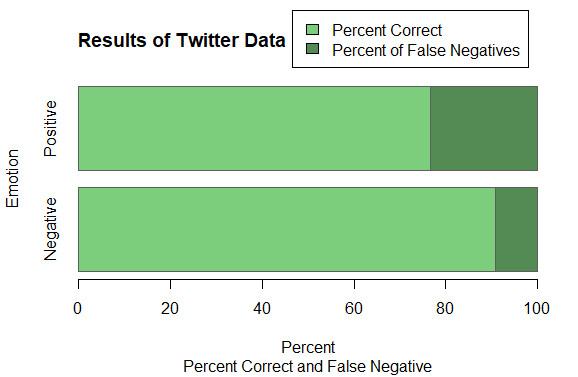
\includegraphics[width = 3.5in]{BarPlotTwitterResults.png}
%	\caption{Barplot of Results of Twitter Data, Positive and Negative Categories}
%\end{figure}


\subsection{Unlabeled Raw Twitter Data Results}

\begin{figure}[h!]

\begin{adjustwidth}{-1in}{-1in}
\begin{subfigure}[]{6cm} \centering \resizebox{\linewidth}{!}{% This file was created by matplotlib2tikz v0.6.18.
\begin{tikzpicture}

\begin{axis}[
axis background/.style={fill=white!89.80392156862746!black},
axis line style={white},
height=6cm,
tick align=outside,
tick pos=left,
title={Sentiment Distribution of Chick-fil-A Twitter Comments},
width=9cm,
x grid style={white},
xlabel={Positive Sentiment Score},
xmajorgrids,
xmin=0, xmax=1,
xtick={0,0.2,0.4,0.6,0.8,1},
xticklabels={0.0,0.2,0.4,0.6,0.8,1.0},
y grid style={white},
ylabel={Percent of Scored Comments},
ymajorgrids,
ymin=0, ymax=7
]
\draw[fill=red,draw opacity=0] (axis cs:0.0219790190458298,0) rectangle (axis cs:0.0463351532816887,0.948521150382389);
\draw[fill=red,draw opacity=0] (axis cs:0.0463351532816887,0) rectangle (axis cs:0.0706912875175476,1.49053335030431);
\draw[fill=red,draw opacity=0] (axis cs:0.0706912875175476,0) rectangle (axis cs:0.0950474217534065,0.813018191075078);
\draw[fill=red,draw opacity=0] (axis cs:0.0950474292039871,0) rectangle (axis cs:0.119403563439846,0.677515159229232);
\draw[fill=red,draw opacity=0] (axis cs:0.119403563439846,0) rectangle (axis cs:0.143759697675705,1.62603588474317);
\draw[fill=red,draw opacity=0] (axis cs:0.143759697675705,0) rectangle (axis cs:0.168115824460983,0.271006146592908);
\draw[fill=red,draw opacity=0] (axis cs:0.168115824460983,0) rectangle (axis cs:0.192471966147423,1.21952691355738);
\draw[fill=red,draw opacity=0] (axis cs:0.192471966147423,0) rectangle (axis cs:0.216828092932701,0.813018439778725);
\draw[fill=red,draw opacity=0] (axis cs:0.216828107833862,0) rectangle (axis cs:0.241184249520302,0.813017942371583);
\draw[fill=red,draw opacity=0] (axis cs:0.241184234619141,0) rectangle (axis cs:0.265540361404419,0.94852151307518);
\draw[fill=red,draw opacity=0] (axis cs:0.265540361404419,0) rectangle (axis cs:0.289896488189697,0.813018439778725);
\draw[fill=red,draw opacity=0] (axis cs:0.289896488189697,0) rectangle (axis cs:0.314252644777298,1.35502907494175);
\draw[fill=red,draw opacity=0] (axis cs:0.314252644777298,0) rectangle (axis cs:0.338608771562576,0.271006146592908);
\draw[fill=red,draw opacity=0] (axis cs:0.338608771562576,0) rectangle (axis cs:0.362964898347855,0.542012293185817);
\draw[fill=red,draw opacity=0] (axis cs:0.362964898347855,0) rectangle (axis cs:0.387321025133133,0.813018439778725);
\draw[fill=red,draw opacity=0] (axis cs:0.387321054935455,0) rectangle (axis cs:0.411677211523056,0.27100581498835);
\draw[fill=red,draw opacity=0] (axis cs:0.411677181720734,0) rectangle (axis cs:0.436033308506012,1.08402458637163);
\draw[fill=red,draw opacity=0] (axis cs:0.436033308506012,0) rectangle (axis cs:0.46038943529129,0.542012293185817);
\draw[fill=red,draw opacity=0] (axis cs:0.46038943529129,0) rectangle (axis cs:0.484745562076569,0.406509219889363);
\draw[fill=red,draw opacity=0] (axis cs:0.484745562076569,0) rectangle (axis cs:0.509101688861847,0.677515366482271);
\draw[fill=red,draw opacity=0] (axis cs:0.509101688861847,0) rectangle (axis cs:0.533457815647125,0);
\draw[fill=red,draw opacity=0] (axis cs:0.53345787525177,0) rectangle (axis cs:0.557814061641693,0.677513708461508);
\draw[fill=red,draw opacity=0] (axis cs:0.557814002037048,0) rectangle (axis cs:0.582170128822327,1.08402458637163);
\draw[fill=red,draw opacity=0] (axis cs:0.582170128822327,0) rectangle (axis cs:0.606526255607605,0.135503073296454);
\draw[fill=red,draw opacity=0] (axis cs:0.606526255607605,0) rectangle (axis cs:0.630882382392883,0.271006146592908);
\draw[fill=red,draw opacity=0] (axis cs:0.630882382392883,0) rectangle (axis cs:0.655238509178162,0.271006146592908);
\draw[fill=red,draw opacity=0] (axis cs:0.655238509178162,0) rectangle (axis cs:0.67959463596344,0.813018439778725);
\draw[fill=red,draw opacity=0] (axis cs:0.67959463596344,0) rectangle (axis cs:0.703950762748718,0.813018439778725);
\draw[fill=red,draw opacity=0] (axis cs:0.703950762748718,0) rectangle (axis cs:0.728306949138641,0.542010966769206);
\draw[fill=red,draw opacity=0] (axis cs:0.728306949138641,0) rectangle (axis cs:0.75266307592392,0.542012293185817);
\draw[fill=red,draw opacity=0] (axis cs:0.75266307592392,0) rectangle (axis cs:0.777019202709198,0.813018439778725);
\draw[fill=red,draw opacity=0] (axis cs:0.777019202709198,0) rectangle (axis cs:0.801375329494476,0.677515366482271);
\draw[fill=red,draw opacity=0] (axis cs:0.801375329494476,0) rectangle (axis cs:0.825731456279755,1.08402458637163);
\draw[fill=red,draw opacity=0] (axis cs:0.825731456279755,0) rectangle (axis cs:0.850087583065033,1.7615399528539);
\draw[fill=red,draw opacity=0] (axis cs:0.850087583065033,0) rectangle (axis cs:0.874443709850311,1.21952765966809);
\draw[fill=red,draw opacity=0] (axis cs:0.874443709850311,0) rectangle (axis cs:0.89879983663559,1.490533806261);
\draw[fill=red,draw opacity=0] (axis cs:0.898799896240234,0) rectangle (axis cs:0.923156082630157,1.62603290030762);
\draw[fill=red,draw opacity=0] (axis cs:0.923156023025513,0) rectangle (axis cs:0.947512149810791,2.57455839263263);
\draw[fill=red,draw opacity=0] (axis cs:0.947512149810791,0) rectangle (axis cs:0.971868276596069,3.2520737591149);
\draw[fill=red,draw opacity=0] (axis cs:0.971868276596069,0) rectangle (axis cs:0.996224403381348,5.01361371196881);
\path [draw=white, fill opacity=0] (axis cs:0,0)
--(axis cs:0,7);

\path [draw=white, fill opacity=0] (axis cs:1,0)
--(axis cs:1,7);

\path [draw=white, fill opacity=0] (axis cs:0,0)
--(axis cs:1,0);

\path [draw=white, fill opacity=0] (axis cs:0,1)
--(axis cs:1,1);

\end{axis}
\label{chickt}
\end{tikzpicture} }  \label{fig:subfig8} \end{subfigure} \begin{subfigure}[]{6cm} \centering \resizebox{\linewidth}{!}{ % This file was created by matplotlib2tikz v0.6.18.
\begin{tikzpicture}

\definecolor{color0}{rgb}{0.580392156862745,0,0.827450980392157}

\begin{axis}[
axis background/.style={fill=white!89.80392156862746!black},
axis line style={white},
height=6cm,
tick align=outside,
tick pos=left,
title={Sentiment Distribution of Taco Bell Twitter Comments},
width=9cm,
x grid style={white},
xlabel={Positive Sentiment Score},
xmajorgrids,
xmin=0, xmax=1,
xtick={0,0.2,0.4,0.6,0.8,1},
xticklabels={0.0,0.2,0.4,0.6,0.8,1.0},
y grid style={white},
ylabel={Percent of Scored Comments},
ymajorgrids,
ymin=0, ymax=7
]
\draw[fill=color0,draw opacity=0] (axis cs:0.0242587197571993,0) rectangle (axis cs:0.048572301864624,0.376704460881885);
\draw[fill=color0,draw opacity=0] (axis cs:0.048572301864624,0) rectangle (axis cs:0.0728858858346939,0.616425386995312);
\draw[fill=color0,draw opacity=0] (axis cs:0.0728858858346939,0) rectangle (axis cs:0.0971994623541832,0.513687979909073);
\draw[fill=color0,draw opacity=0] (axis cs:0.0971994623541832,0) rectangle (axis cs:0.121513046324253,0.924638080492968);
\draw[fill=color0,draw opacity=0] (axis cs:0.121513053774834,0) rectangle (axis cs:0.145826637744904,0.513687979909073);
\draw[fill=color0,draw opacity=0] (axis cs:0.145826637744904,0) rectangle (axis cs:0.170140221714973,0.684917096661458);
\draw[fill=color0,draw opacity=0] (axis cs:0.170140206813812,0) rectangle (axis cs:0.194453790783882,0.205475128998437);
\draw[fill=color0,draw opacity=0] (axis cs:0.194453805685043,0) rectangle (axis cs:0.218767389655113,0.71916295149453);
\draw[fill=color0,draw opacity=0] (axis cs:0.218767374753952,0) rectangle (axis cs:0.243080958724022,0.513687822496093);
\draw[fill=color0,draw opacity=0] (axis cs:0.243080973625183,0) rectangle (axis cs:0.267394542694092,0.890392225659895);
\draw[fill=color0,draw opacity=0] (axis cs:0.267394542694092,0) rectangle (axis cs:0.291708111763,0.616425764786579);
\draw[fill=color0,draw opacity=0] (axis cs:0.291708111763,0) rectangle (axis cs:0.316021710634232,0.239720836912864);
\draw[fill=color0,draw opacity=0] (axis cs:0.316021710634232,0) rectangle (axis cs:0.34033527970314,0.753409268072485);
\draw[fill=color0,draw opacity=0] (axis cs:0.34033527970314,0) rectangle (axis cs:0.364648848772049,0.479442261500672);
\draw[fill=color0,draw opacity=0] (axis cs:0.364648878574371,0) rectangle (axis cs:0.388962477445602,0.308212504602254);
\draw[fill=color0,draw opacity=0] (axis cs:0.38896244764328,0) rectangle (axis cs:0.413276016712189,0.650671640608055);
\draw[fill=color0,draw opacity=0] (axis cs:0.413276016712189,0) rectangle (axis cs:0.43758961558342,0.582179175359813);
\draw[fill=color0,draw opacity=0] (axis cs:0.43758961558342,0) rectangle (axis cs:0.461903184652328,0.684917516429532);
\draw[fill=color0,draw opacity=0] (axis cs:0.461903184652328,0) rectangle (axis cs:0.486216753721237,0.856146895536915);
\draw[fill=color0,draw opacity=0] (axis cs:0.48621678352356,0) rectangle (axis cs:0.510530352592468,1.02737501534085);
\draw[fill=color0,draw opacity=0] (axis cs:0.510530352592468,0) rectangle (axis cs:0.534843921661377,0.650671640608055);
\draw[fill=color0,draw opacity=0] (axis cs:0.534843921661377,0) rectangle (axis cs:0.559157490730286,0.342458758214766);
\draw[fill=color0,draw opacity=0] (axis cs:0.559157490730286,0) rectangle (axis cs:0.583471119403839,3.15061285185748);
\draw[fill=color0,draw opacity=0] (axis cs:0.583471119403839,0) rectangle (axis cs:0.607784688472748,0.479442261500672);
\draw[fill=color0,draw opacity=0] (axis cs:0.607784688472748,0) rectangle (axis cs:0.632098257541656,0.616425764786579);
\draw[fill=color0,draw opacity=0] (axis cs:0.632098257541656,0) rectangle (axis cs:0.656411826610565,1.47257266032349);
\draw[fill=color0,draw opacity=0] (axis cs:0.656411826610565,0) rectangle (axis cs:0.680725395679474,0.958884523001344);
\draw[fill=color0,draw opacity=0] (axis cs:0.680725336074829,0) rectangle (axis cs:0.705038964748383,0.821899004832387);
\draw[fill=color0,draw opacity=0] (axis cs:0.705039024353027,0) rectangle (axis cs:0.729352593421936,1.13011390210873);
\draw[fill=color0,draw opacity=0] (axis cs:0.729352593421936,0) rectangle (axis cs:0.753666162490845,0.719163392251008);
\draw[fill=color0,draw opacity=0] (axis cs:0.753666162490845,0) rectangle (axis cs:0.777979731559753,1.54106441196645);
\draw[fill=color0,draw opacity=0] (axis cs:0.777979731559753,0) rectangle (axis cs:0.802293300628662,0.958884523001344);
\draw[fill=color0,draw opacity=0] (axis cs:0.802293300628662,0) rectangle (axis cs:0.826606929302216,0.890390588568419);
\draw[fill=color0,draw opacity=0] (axis cs:0.826606929302216,0) rectangle (axis cs:0.850920498371124,2.22598192839598);
\draw[fill=color0,draw opacity=0] (axis cs:0.850920498371124,0) rectangle (axis cs:0.875234067440033,1.1643597779302);
\draw[fill=color0,draw opacity=0] (axis cs:0.875234067440033,0) rectangle (axis cs:0.899547636508942,1.23285152957316);
\draw[fill=color0,draw opacity=0] (axis cs:0.899547636508942,0) rectangle (axis cs:0.92386120557785,2.02050667346712);
\draw[fill=color0,draw opacity=0] (axis cs:0.923861145973206,0) rectangle (axis cs:0.948174774646759,2.15748488768502);
\draw[fill=color0,draw opacity=0] (axis cs:0.948174834251404,0) rectangle (axis cs:0.972488403320312,1.50681853614497);
\draw[fill=color0,draw opacity=0] (axis cs:0.972488403320312,0) rectangle (axis cs:0.996801972389221,4.93140611829263);
\path [draw=white, fill opacity=0] (axis cs:0,0)
--(axis cs:0,7);

\path [draw=white, fill opacity=0] (axis cs:1,0)
--(axis cs:1,7);

\path [draw=white, fill opacity=0] (axis cs:0,0)
--(axis cs:1,0);

\path [draw=white, fill opacity=0] (axis cs:0,1)
--(axis cs:1,1);

\end{axis}
\label{tacot}
\end{tikzpicture}\hfill }  \label{fig:subfig9} \end{subfigure} \begin{subfigure}[]{6cm} \centering \resizebox{\linewidth}{!}{ 
% This file was created by matplotlib2tikz v0.6.18.
\begin{tikzpicture}

\definecolor{color0}{rgb}{0.250980392156863,0.87843137254902,0.815686274509804}

\begin{axis}[
axis background/.style={fill=white!89.80392156862746!black},
axis line style={white},
height=4cm,
tick align=outside,
tick pos=left,
title={Sentiment Distribution of Pal's},
width=6cm,
x grid style={white},
xlabel={Positive Sentiment Score},
xmajorgrids,
xmin=0, xmax=1,
xtick={0,0.2,0.4,0.6,0.8,1},
xticklabels={0.0,0.2,0.4,0.6,0.8,1.0},
y grid style={white},
ylabel={Percent},
ymajorgrids,
ymin=0, ymax=7
]
\draw[fill=color0,draw opacity=0] (axis cs:0.0140848532319069,0) rectangle (axis cs:0.0386082269251347,0.520562855930947);
\draw[fill=color0,draw opacity=0] (axis cs:0.0386082231998444,0) rectangle (axis cs:0.0631316006183624,0.983285394536234);
\draw[fill=color0,draw opacity=0] (axis cs:0.0631316006183624,0) rectangle (axis cs:0.0876549705862999,0.404882282784379);
\draw[fill=color0,draw opacity=0] (axis cs:0.0876549705862999,0) rectangle (axis cs:0.112178348004818,0.694083702471243);
\draw[fill=color0,draw opacity=0] (axis cs:0.112178340554237,0) rectangle (axis cs:0.136701703071594,0.925445217792865);
\draw[fill=color0,draw opacity=0] (axis cs:0.136701717972755,0) rectangle (axis cs:0.161225095391273,1.21464647932467);
\draw[fill=color0,draw opacity=0] (axis cs:0.161225095391273,0) rectangle (axis cs:0.185748472809792,0.867604628089053);
\draw[fill=color0,draw opacity=0] (axis cs:0.18574845790863,0) rectangle (axis cs:0.210271820425987,1.56168927949091);
\draw[fill=color0,draw opacity=0] (axis cs:0.210271835327148,0) rectangle (axis cs:0.234795212745667,0.925444936628323);
\draw[fill=color0,draw opacity=0] (axis cs:0.234795212745667,0) rectangle (axis cs:0.259318590164185,1.21464647932467);
\draw[fill=color0,draw opacity=0] (axis cs:0.259318590164185,0) rectangle (axis cs:0.283841967582703,1.27248678786394);
\draw[fill=color0,draw opacity=0] (axis cs:0.283841967582703,0) rectangle (axis cs:0.308365345001221,0.751924011010513);
\draw[fill=color0,draw opacity=0] (axis cs:0.308365345001221,0) rectangle (axis cs:0.332888722419739,0.404882159774892);
\draw[fill=color0,draw opacity=0] (axis cs:0.332888722419739,0) rectangle (axis cs:0.357412070035934,0.636244167135168);
\draw[fill=color0,draw opacity=0] (axis cs:0.357412070035934,0) rectangle (axis cs:0.381935447454453,1.04112555370686);
\draw[fill=color0,draw opacity=0] (axis cs:0.381935447454453,0) rectangle (axis cs:0.406458824872971,0.404882159774892);
\draw[fill=color0,draw opacity=0] (axis cs:0.406458824872971,0) rectangle (axis cs:0.430982202291489,1.33032709640321);
\draw[fill=color0,draw opacity=0] (axis cs:0.430982202291489,0) rectangle (axis cs:0.455505579710007,0.347041851235621);
\draw[fill=color0,draw opacity=0] (axis cs:0.455505579710007,0) rectangle (axis cs:0.480028957128525,0.404882159774892);
\draw[fill=color0,draw opacity=0] (axis cs:0.480028927326202,0) rectangle (axis cs:0.504552245140076,0.751924924796108);
\draw[fill=color0,draw opacity=0] (axis cs:0.50455230474472,0) rectangle (axis cs:0.529075682163239,0.11568061707854);
\draw[fill=color0,draw opacity=0] (axis cs:0.529075682163239,0) rectangle (axis cs:0.553599059581757,0.636243393931972);
\draw[fill=color0,draw opacity=0] (axis cs:0.553599059581757,0) rectangle (axis cs:0.578122437000275,2.19793172449227);
\draw[fill=color0,draw opacity=0] (axis cs:0.578122437000275,0) rectangle (axis cs:0.602645814418793,0.347041851235621);
\draw[fill=color0,draw opacity=0] (axis cs:0.602645814418793,0) rectangle (axis cs:0.627169191837311,0.751924011010513);
\draw[fill=color0,draw opacity=0] (axis cs:0.627169191837311,0) rectangle (axis cs:0.651692569255829,0.694083702471243);
\draw[fill=color0,draw opacity=0] (axis cs:0.651692569255829,0) rectangle (axis cs:0.676215946674347,0.751924011010513);
\draw[fill=color0,draw opacity=0] (axis cs:0.676215946674347,0) rectangle (axis cs:0.700739324092865,0.404882159774892);
\draw[fill=color0,draw opacity=0] (axis cs:0.700739324092865,0) rectangle (axis cs:0.725262701511383,2.25577203303154);
\draw[fill=color0,draw opacity=0] (axis cs:0.725262701511383,0) rectangle (axis cs:0.749786078929901,0.636243393931972);
\draw[fill=color0,draw opacity=0] (axis cs:0.749786078929901,0) rectangle (axis cs:0.774309456348419,0.694083702471243);
\draw[fill=color0,draw opacity=0] (axis cs:0.774309456348419,0) rectangle (axis cs:0.798832833766937,1.09896586224613);
\draw[fill=color0,draw opacity=0] (axis cs:0.798832893371582,0) rectangle (axis cs:0.823356211185455,0.925447185949444);
\draw[fill=color0,draw opacity=0] (axis cs:0.823356151580811,0) rectangle (axis cs:0.847879528999329,3.00769604404205);
\draw[fill=color0,draw opacity=0] (axis cs:0.847879528999329,0) rectangle (axis cs:0.872402906417847,0.694083702471243);
\draw[fill=color0,draw opacity=0] (axis cs:0.872402906417847,0) rectangle (axis cs:0.896926283836365,1.1568061707854);
\draw[fill=color0,draw opacity=0] (axis cs:0.896926283836365,0) rectangle (axis cs:0.921449661254883,0.925444936628323);
\draw[fill=color0,draw opacity=0] (axis cs:0.921449661254883,0) rectangle (axis cs:0.945973038673401,1.5616883305603);
\draw[fill=color0,draw opacity=0] (axis cs:0.945973038673401,0) rectangle (axis cs:0.970496416091919,1.27248678786394);
\draw[fill=color0,draw opacity=0] (axis cs:0.970496416091919,0) rectangle (axis cs:0.995019793510437,3.99098128920964);
\path [draw=white, fill opacity=0] (axis cs:0,0)
--(axis cs:0,7);

\path [draw=white, fill opacity=0] (axis cs:1,0)
--(axis cs:1,7);

\path [draw=white, fill opacity=0] (axis cs:0,0)
--(axis cs:1,0);

\path [draw=white, fill opacity=0] (axis cs:0,1)
--(axis cs:1,1);

\end{axis}

\end{tikzpicture} }  \label{fig:subfig10} \end{subfigure}  \label{fig:subfig1.a.4} 
\begin{subfigure}[]{6cm} \centering \resizebox{\linewidth}{!}{% This file was created by matplotlib2tikz v0.6.18.
\begin{tikzpicture}

\definecolor{color0}{rgb}{0.698039215686274,0.133333333333333,0.133333333333333}

\begin{axis}[
axis background/.style={fill=white!89.80392156862746!black},
axis line style={white},
height=4cm,
tick align=outside,
tick pos=left,
title={Sentiment Distribution of Chipotle Twitter Comments},
width=6cm,
x grid style={white},
xlabel={Positive Sentiment Score},
xmajorgrids,
xmin=0, xmax=1,
xtick={0,0.2,0.4,0.6,0.8,1},
xticklabels={0.0,0.2,0.4,0.6,0.8,1.0},
y grid style={white},
ylabel={Percent of Scored Comments},
ymajorgrids,
ymin=0, ymax=7
]
\draw[fill=color0,draw opacity=0] (axis cs:0.0257699713110924,0) rectangle (axis cs:0.0492510721087456,4.96853520312578);
\draw[fill=color0,draw opacity=0] (axis cs:0.0492510721087456,0) rectangle (axis cs:0.0727321654558182,4.96853638551765);
\draw[fill=color0,draw opacity=0] (axis cs:0.0727321654558182,0) rectangle (axis cs:0.0962132662534714,4.96853480899528);
\draw[fill=color0,draw opacity=0] (axis cs:0.0962132662534714,0) rectangle (axis cs:0.119694359600544,3.54895456108404);
\draw[fill=color0,draw opacity=0] (axis cs:0.119694352149963,0) rectangle (axis cs:0.143175452947617,0);
\draw[fill=color0,draw opacity=0] (axis cs:0.143175452947617,0) rectangle (axis cs:0.16665655374527,0.709790686999325);
\draw[fill=color0,draw opacity=0] (axis cs:0.16665655374527,0) rectangle (axis cs:0.190137654542923,1.41958137399865);
\draw[fill=color0,draw opacity=0] (axis cs:0.190137654542923,0) rectangle (axis cs:0.213618755340576,1.41958137399865);
\draw[fill=color0,draw opacity=0] (axis cs:0.213618755340576,0) rectangle (axis cs:0.237099841237068,2.83916454973773);
\draw[fill=color0,draw opacity=0] (axis cs:0.237099826335907,0) rectangle (axis cs:0.260580956935883,0);
\draw[fill=color0,draw opacity=0] (axis cs:0.260580956935883,0) rectangle (axis cs:0.284062027931213,3.54895793935056);
\draw[fill=color0,draw opacity=0] (axis cs:0.284062027931213,0) rectangle (axis cs:0.307543128728867,1.41958137399865);
\draw[fill=color0,draw opacity=0] (axis cs:0.307543098926544,0) rectangle (axis cs:0.331024199724197,2.12937206099798);
\draw[fill=color0,draw opacity=0] (axis cs:0.33102422952652,0) rectangle (axis cs:0.354505330324173,0);
\draw[fill=color0,draw opacity=0] (axis cs:0.354505300521851,0) rectangle (axis cs:0.377986401319504,0);
\draw[fill=color0,draw opacity=0] (axis cs:0.377986431121826,0) rectangle (axis cs:0.401467531919479,0);
\draw[fill=color0,draw opacity=0] (axis cs:0.401467502117157,0) rectangle (axis cs:0.42494860291481,0);
\draw[fill=color0,draw opacity=0] (axis cs:0.424948632717133,0) rectangle (axis cs:0.448429733514786,0);
\draw[fill=color0,draw opacity=0] (axis cs:0.448429703712463,0) rectangle (axis cs:0.471910804510117,0);
\draw[fill=color0,draw opacity=0] (axis cs:0.471910834312439,0) rectangle (axis cs:0.49539190530777,0);
\draw[fill=color0,draw opacity=0] (axis cs:0.49539190530777,0) rectangle (axis cs:0.518873035907745,0);
\draw[fill=color0,draw opacity=0] (axis cs:0.518872976303101,0) rectangle (axis cs:0.542354047298431,0);
\draw[fill=color0,draw opacity=0] (axis cs:0.542354106903076,0) rectangle (axis cs:0.565835237503052,0.709789786130826);
\draw[fill=color0,draw opacity=0] (axis cs:0.565835237503052,0) rectangle (axis cs:0.589316308498383,0);
\draw[fill=color0,draw opacity=0] (axis cs:0.589316248893738,0) rectangle (axis cs:0.612797319889069,0);
\draw[fill=color0,draw opacity=0] (axis cs:0.612797379493713,0) rectangle (axis cs:0.636278510093689,0);
\draw[fill=color0,draw opacity=0] (axis cs:0.636278510093689,0) rectangle (axis cs:0.65975958108902,0.709791587870111);
\draw[fill=color0,draw opacity=0] (axis cs:0.65975958108902,0) rectangle (axis cs:0.683240711688995,0);
\draw[fill=color0,draw opacity=0] (axis cs:0.683240652084351,0) rectangle (axis cs:0.706721723079681,2.83916635148044);
\draw[fill=color0,draw opacity=0] (axis cs:0.706721782684326,0) rectangle (axis cs:0.730202913284302,0);
\draw[fill=color0,draw opacity=0] (axis cs:0.730202913284302,0) rectangle (axis cs:0.753683984279633,0);
\draw[fill=color0,draw opacity=0] (axis cs:0.753683924674988,0) rectangle (axis cs:0.777164995670319,0.709791587870111);
\draw[fill=color0,draw opacity=0] (axis cs:0.777165055274963,0) rectangle (axis cs:0.800646185874939,0);
\draw[fill=color0,draw opacity=0] (axis cs:0.800646185874939,0) rectangle (axis cs:0.82412725687027,0.709791587870111);
\draw[fill=color0,draw opacity=0] (axis cs:0.82412725687027,0) rectangle (axis cs:0.847608387470245,1.41957957226165);
\draw[fill=color0,draw opacity=0] (axis cs:0.847608327865601,0) rectangle (axis cs:0.871089398860931,0.709791587870111);
\draw[fill=color0,draw opacity=0] (axis cs:0.871089458465576,0) rectangle (axis cs:0.894570589065552,1.41957957226165);
\draw[fill=color0,draw opacity=0] (axis cs:0.894570589065552,0) rectangle (axis cs:0.918051660060883,0);
\draw[fill=color0,draw opacity=0] (axis cs:0.918051660060883,0) rectangle (axis cs:0.941532790660858,0);
\draw[fill=color0,draw opacity=0] (axis cs:0.941532731056213,0) rectangle (axis cs:0.965013802051544,1.41958317574022);
\path [draw=white, fill opacity=0] (axis cs:0,0)
--(axis cs:0,7);

\path [draw=white, fill opacity=0] (axis cs:1,0)
--(axis cs:1,7);

\path [draw=white, fill opacity=0] (axis cs:0,0)
--(axis cs:1,0);

\path [draw=white, fill opacity=0] (axis cs:0,1)
--(axis cs:1,1);

\end{axis}

\end{tikzpicture} }  \label{fig:subfig8} \end{subfigure}
\begin{subfigure}[]{6cm} \centering \resizebox{\linewidth}{!}{% This file was created by matplotlib2tikz v0.6.18.
\begin{tikzpicture}

\definecolor{color0}{rgb}{0.419607843137255,0.556862745098039,0.137254901960784}

\begin{axis}[
axis background/.style={fill=white!89.80392156862746!black},
axis line style={white},
height=4cm,
tick align=outside,
tick pos=left,
title={Sentiment Distribution of Panera Twitter Comments},
width=6cm,
x grid style={white},
xlabel={Positive Sentiment Score},
xmajorgrids,
xmin=0, xmax=1,
xtick={0,0.2,0.4,0.6,0.8,1},
xticklabels={0.0,0.2,0.4,0.6,0.8,1.0},
y grid style={white},
ylabel={Percent of Scored Comments},
ymajorgrids,
ymin=0, ymax=7
]
\draw[fill=color0,draw opacity=0] (axis cs:0.0268173981457949,0) rectangle (axis cs:0.0509582459926605,0.56585136775584);
\draw[fill=color0,draw opacity=0] (axis cs:0.0509582459926605,0) rectangle (axis cs:0.0750990957021713,1.92226990004779);
\draw[fill=color0,draw opacity=0] (axis cs:0.0750990957021713,0) rectangle (axis cs:0.0992399379611015,0.969257516348745);
\draw[fill=color0,draw opacity=0] (axis cs:0.0992399379611015,0) rectangle (axis cs:0.123380787670612,0.958427527629459);
\draw[fill=color0,draw opacity=0] (axis cs:0.123380795121193,0) rectangle (axis cs:0.147521644830704,0.435895140033933);
\draw[fill=color0,draw opacity=0] (axis cs:0.147521644830704,0) rectangle (axis cs:0.171662494540215,0.69580755536941);
\draw[fill=color0,draw opacity=0] (axis cs:0.171662479639053,0) rectangle (axis cs:0.195803329348564,0.411528203953892);
\draw[fill=color0,draw opacity=0] (axis cs:0.195803329348564,0) rectangle (axis cs:0.219944164156914,0.974672663621713);
\draw[fill=color0,draw opacity=0] (axis cs:0.219944179058075,0) rectangle (axis cs:0.244085028767586,0.552314168464434);
\draw[fill=color0,draw opacity=0] (axis cs:0.244085013866425,0) rectangle (axis cs:0.268225848674774,0.414235882039228);
\draw[fill=color0,draw opacity=0] (axis cs:0.268225848674774,0) rectangle (axis cs:0.292366713285446,0.281571755218332);
\draw[fill=color0,draw opacity=0] (axis cs:0.292366713285446,0) rectangle (axis cs:0.316507548093796,0.140786051412025);
\draw[fill=color0,draw opacity=0] (axis cs:0.316507577896118,0) rectangle (axis cs:0.34064844250679,0.682270022259805);
\draw[fill=color0,draw opacity=0] (axis cs:0.340648412704468,0) rectangle (axis cs:0.364789247512817,0.143493475477641);
\draw[fill=color0,draw opacity=0] (axis cs:0.364789247512817,0) rectangle (axis cs:0.388930082321167,0.148908323608873);
\draw[fill=color0,draw opacity=0] (axis cs:0.388930082321167,0) rectangle (axis cs:0.413070946931839,0.679562601536552);
\draw[fill=color0,draw opacity=0] (axis cs:0.413070946931839,0) rectangle (axis cs:0.437211781740189,0.414235882039228);
\draw[fill=color0,draw opacity=0] (axis cs:0.437211811542511,0) rectangle (axis cs:0.461352676153183,0.955719515308377);
\draw[fill=color0,draw opacity=0] (axis cs:0.461352646350861,0) rectangle (axis cs:0.48549348115921,0.546899661254406);
\draw[fill=color0,draw opacity=0] (axis cs:0.48549348115921,0) rectangle (axis cs:0.50963431596756,0.693100560797663);
\draw[fill=color0,draw opacity=0] (axis cs:0.50963431596756,0) rectangle (axis cs:0.533775150775909,0.560436781582485);
\draw[fill=color0,draw opacity=0] (axis cs:0.533775210380554,0) rectangle (axis cs:0.557916104793549,0.276156572851675);
\draw[fill=color0,draw opacity=0] (axis cs:0.557916045188904,0) rectangle (axis cs:0.582056879997253,0.817642067815993);
\draw[fill=color0,draw opacity=0] (axis cs:0.582056879997253,0) rectangle (axis cs:0.606197714805603,0.146200899543257);
\draw[fill=color0,draw opacity=0] (axis cs:0.606197714805603,0) rectangle (axis cs:0.630338549613953,0.820349491881609);
\draw[fill=color0,draw opacity=0] (axis cs:0.630338549613953,0) rectangle (axis cs:0.654479384422302,1.0910918984432);
\draw[fill=color0,draw opacity=0] (axis cs:0.654479384422302,0) rectangle (axis cs:0.678620278835297,0.85825130974491);
\draw[fill=color0,draw opacity=0] (axis cs:0.678620278835297,0) rectangle (axis cs:0.702761113643646,0.684978288600815);
\draw[fill=color0,draw opacity=0] (axis cs:0.702761113643646,0) rectangle (axis cs:0.726901948451996,0.292401799086514);
\draw[fill=color0,draw opacity=0] (axis cs:0.726901948451996,0) rectangle (axis cs:0.751042783260345,0.546899661254406);
\draw[fill=color0,draw opacity=0] (axis cs:0.751042783260345,0) rectangle (axis cs:0.775183618068695,0.0297816647217746);
\draw[fill=color0,draw opacity=0] (axis cs:0.775183618068695,0) rectangle (axis cs:0.799324452877045,1.24000022205207);
\draw[fill=color0,draw opacity=0] (axis cs:0.799324512481689,0) rectangle (axis cs:0.823465406894684,2.47187206876058);
\draw[fill=color0,draw opacity=0] (axis cs:0.823465347290039,0) rectangle (axis cs:0.847606182098389,1.23729279798645);
\draw[fill=color0,draw opacity=0] (axis cs:0.847606182098389,0) rectangle (axis cs:0.871747016906738,1.64340640782883);
\draw[fill=color0,draw opacity=0] (axis cs:0.871747016906738,0) rectangle (axis cs:0.895887851715088,1.53240202113858);
\draw[fill=color0,draw opacity=0] (axis cs:0.895887851715088,0) rectangle (axis cs:0.920028686523438,1.9276859347185);
\draw[fill=color0,draw opacity=0] (axis cs:0.920028686523438,0) rectangle (axis cs:0.944169580936432,3.14331157922347);
\draw[fill=color0,draw opacity=0] (axis cs:0.944169580936432,0) rectangle (axis cs:0.968310415744781,3.97991337645533);
\draw[fill=color0,draw opacity=0] (axis cs:0.968310415744781,0) rectangle (axis cs:0.992451250553131,5.53668221418445);
\path [draw=white, fill opacity=0] (axis cs:0,0)
--(axis cs:0,7);

\path [draw=white, fill opacity=0] (axis cs:1,0)
--(axis cs:1,7);

\path [draw=white, fill opacity=0] (axis cs:0,0)
--(axis cs:1,0);

\path [draw=white, fill opacity=0] (axis cs:0,1)
--(axis cs:1,1);

\end{axis}

\end{tikzpicture} }  \label{fig:subfig8} \end{subfigure}
\end{adjustwidth}
\end{figure}

For the final step in this project we tested our model on a few different sets of raw unlabeled twitter data. The data sets were tweets at a few different restaurants. We chose Panera, Taco Bell, Chick-Fil-A, and Pal's. The model which trained on the labeled twitter data, then went through a set of the raw twitter data and for each tweet gave a percent positive score. We then made a histogram of this data. So we have a histogram of "positivity" for each restaurants tweets. First we look at the results from Panera tweets. 



As we can see from the Panera Results (\cref{fig:Paneratt}). The model predicted mostly positive responses. This is not surprising, Panera has a good reputation for great food and customer service. Obviously there are some less positive or negative reviews, but the majority of the reviews are positive.

Next we look at the results for tweets at the fast food chain Pal's.



From figure \cref{fig:chicktt} we can see that the majority of Pal's tweets have a positive sentiment score, which is good. This histogram is not as heavily skewed as the Panera histogram, so there may be slightly more negative tweets as compared to Panera, but overall Pal's is doing well from the customers standpoint. 

Next we look at the results from Taco Bell tweets.



In figure \cref{fig:tacott} we see that Taco Bell again is mostly in the positive score range, but the histogram does even off around $.06$. Overall it would appear that Taco Bell is meeting customer expectations. 

Finally we look at the results for Chick-Fil-A.


%\vspace{-2in}
%\input{Chick-Fil-A.tex}

From figure \cref{fig:chicktt} we see a high percentage of tweets with positive sentiment. This tells us that Chick-Fil-A is doing well overall. They are meeting customers expectations. They do have some negative tweets, just as the previous restaurants do, but that is to be expected. No business is perfect, so some less than positive reviews are bound to occur. It is interesting to note that there are not as many middling positive tweets, or tweets that fall in the middle of the graph.

Figure \ref{compstat} displays some basic statistical analysis on each restaurant from the raw unlabeled Twitter data. The red bar gives the proportion of positive reviews which were over $0.5$ on the positive sentiment score, the blue bar gives the mean positive sentiment score, and the purple bar shows the median positive sentiment score for each restaurant. As we can see most of the restaurants are positive, each of the bars falls over $0.5$ in this bar graph. The only two exceptions are Chipotle and Comcast, which both have means that are higher than their medians. This is not surprising since we know that a mean will be pulled toward the outliers. Panera appears to have the most positive statistics of the restaurants, with a median score of $0.8$. 

\begin{figure}[htb]
	\centering
	\caption{Statistical Comparison of Twitter Restaurants}
	% This file was created by matplotlib2tikz v0.6.18.
\begin{tikzpicture}

\definecolor{color0}{rgb}{0.886274509803922,0.290196078431373,0.2}
\definecolor{color1}{rgb}{0.203921568627451,0.541176470588235,0.741176470588235}
\definecolor{color2}{rgb}{0.596078431372549,0.556862745098039,0.835294117647059}

\begin{axis}[
axis background/.style={fill=white!89.80392156862746!black},
axis line style={white},
height=4cm,
legend cell align={left},
legend columns=3,
legend entries={{Percent Positive},{Mean Score},{Median Score}},
legend style={at={(0.5,1.05)}, anchor=north, draw=white!80.0!black, fill=white!89.80392156862746!black},
tick align=outside,
tick pos=left,
title={@ Fast Food Company Sentiment Comparison},
width=6cm,
x grid style={white},
xmajorgrids,
xmin=-0.5, xmax=12.5,
xtick={0,1,2,3,4,5,6,7,8,9,10,11,12},
xticklabel style = {rotate=90},
xticklabels={Chick-fil-A,Panera,Chipotle,Pal's,Taco Bell,Comcast,McDonalds's,KFC,Steak 'n Shake,Five Guys,Wendys,Subway,Quizno's},
y grid style={white},
ymajorgrids,
ymin=0, ymax=0.839734277129173,
ytick={0,0.1,0.2,0.3,0.4,0.5,0.6,0.7,0.8,0.9},
yticklabels={0.0,0.1,0.2,0.3,0.4,0.5,0.6,0.7,0.8,0.9}
]
\addlegendimage{ybar,ybar legend,fill=color0,draw opacity=0};
\draw[fill=color0,draw opacity=0] (axis cs:-0.25,0) rectangle (axis cs:-0.0833333333333333,0.64026402640264);
\draw[fill=color0,draw opacity=0] (axis cs:0.75,0) rectangle (axis cs:0.916666666666667,0.706209150326797);
\draw[fill=color0,draw opacity=0] (axis cs:1.75,0) rectangle (axis cs:1.91666666666667,0.25);
\draw[fill=color0,draw opacity=0] (axis cs:2.75,0) rectangle (axis cs:2.91666666666667,0.659574468085106);
\draw[fill=color0,draw opacity=0] (axis cs:3.75,0) rectangle (axis cs:3.91666666666667,0.743547044129892);
\draw[fill=color0,draw opacity=0] (axis cs:4.75,0) rectangle (axis cs:4.91666666666667,0.385294117647059);
\draw[fill=color0,draw opacity=0] (axis cs:5.75,0) rectangle (axis cs:5.91666666666667,0.717777777777778);
\draw[fill=color0,draw opacity=0] (axis cs:6.75,0) rectangle (axis cs:6.91666666666667,0.678376268540203);
\draw[fill=color0,draw opacity=0] (axis cs:7.75,0) rectangle (axis cs:7.91666666666667,0.591435185185185);
\draw[fill=color0,draw opacity=0] (axis cs:8.75,0) rectangle (axis cs:8.91666666666667,0.63515625);
\draw[fill=color0,draw opacity=0] (axis cs:9.75,0) rectangle (axis cs:9.91666666666667,0.64);
\draw[fill=color0,draw opacity=0] (axis cs:10.75,0) rectangle (axis cs:10.9166666666667,0.725137039937353);
\draw[fill=color0,draw opacity=0] (axis cs:11.75,0) rectangle (axis cs:11.9166666666667,0.69296875);
\addlegendimage{ybar,ybar legend,fill=color1,draw opacity=0};
\draw[fill=color1,draw opacity=0] (axis cs:-0.0833333333333333,0) rectangle (axis cs:0.0833333333333333,0.62245386838913);
\draw[fill=color1,draw opacity=0] (axis cs:0.916666666666667,0) rectangle (axis cs:1.08333333333333,0.664597392082214);
\draw[fill=color1,draw opacity=0] (axis cs:1.91666666666667,0) rectangle (axis cs:2.08333333333333,0.325299382209778);
\draw[fill=color1,draw opacity=0] (axis cs:2.91666666666667,0) rectangle (axis cs:3.08333333333333,0.617715835571289);
\draw[fill=color1,draw opacity=0] (axis cs:3.91666666666667,0) rectangle (axis cs:4.08333333333333,0.664495289325714);
\draw[fill=color1,draw opacity=0] (axis cs:4.91666666666667,0) rectangle (axis cs:5.08333333333333,0.406776398420334);
\draw[fill=color1,draw opacity=0] (axis cs:5.91666666666667,0) rectangle (axis cs:6.08333333333333,0.665299892425537);
\draw[fill=color1,draw opacity=0] (axis cs:6.91666666666667,0) rectangle (axis cs:7.08333333333333,0.627276062965393);
\draw[fill=color1,draw opacity=0] (axis cs:7.91666666666667,0) rectangle (axis cs:8.08333333333333,0.555412709712982);
\draw[fill=color1,draw opacity=0] (axis cs:8.91666666666667,0) rectangle (axis cs:9.08333333333333,0.605079054832458);
\draw[fill=color1,draw opacity=0] (axis cs:9.91666666666667,0) rectangle (axis cs:10.0833333333333,0.606943249702454);
\draw[fill=color1,draw opacity=0] (axis cs:10.9166666666667,0) rectangle (axis cs:11.0833333333333,0.667344927787781);
\draw[fill=color1,draw opacity=0] (axis cs:11.9166666666667,0) rectangle (axis cs:12.0833333333333,0.649368464946747);
\addlegendimage{ybar,ybar legend,fill=color2,draw opacity=0};
\draw[fill=color2,draw opacity=0] (axis cs:0.0833333333333333,0) rectangle (axis cs:0.25,0.730778276920319);
\draw[fill=color2,draw opacity=0] (axis cs:1.08333333333333,0) rectangle (axis cs:1.25,0.799746930599213);
\draw[fill=color2,draw opacity=0] (axis cs:2.08333333333333,0) rectangle (axis cs:2.25,0.188174426555634);
\draw[fill=color2,draw opacity=0] (axis cs:3.08333333333333,0) rectangle (axis cs:3.25,0.691534161567688);
\draw[fill=color2,draw opacity=0] (axis cs:4.08333333333333,0) rectangle (axis cs:4.25,0.740769445896149);
\draw[fill=color2,draw opacity=0] (axis cs:5.08333333333333,0) rectangle (axis cs:5.25,0.295030832290649);
\draw[fill=color2,draw opacity=0] (axis cs:6.08333333333333,0) rectangle (axis cs:6.25,0.793573141098022);
\draw[fill=color2,draw opacity=0] (axis cs:7.08333333333333,0) rectangle (axis cs:7.25,0.70574164390564);
\draw[fill=color2,draw opacity=0] (axis cs:8.08333333333333,0) rectangle (axis cs:8.25,0.631855547428131);
\draw[fill=color2,draw opacity=0] (axis cs:9.08333333333333,0) rectangle (axis cs:9.25,0.682299554347992);
\draw[fill=color2,draw opacity=0] (axis cs:10.0833333333333,0) rectangle (axis cs:10.25,0.687142729759216);
\draw[fill=color2,draw opacity=0] (axis cs:11.0833333333333,0) rectangle (axis cs:11.25,0.788477540016174);
\draw[fill=color2,draw opacity=0] (axis cs:12.0833333333333,0) rectangle (axis cs:12.25,0.7463259100914);
\path [draw=white, fill opacity=0] (axis cs:0,0)
--(axis cs:0,0.839734277129173);

\path [draw=white, fill opacity=0] (axis cs:1,0)
--(axis cs:1,0.839734277129173);

\path [draw=white, fill opacity=0] (axis cs:-0.5,0)
--(axis cs:12.5,0);

\path [draw=white, fill opacity=0] (axis cs:-0.5,1)
--(axis cs:12.5,1);

\end{axis}

\end{tikzpicture}
	\label{compstat}
\end{figure}


\subsection{Mcdonalds Service Failure Sentiment Results}

The McDonalds Service failure is a labeled data set that contains just over $1500$ reviews. The reviews are of Mcdonalds restaurants in different locations around the United States. The Mcdonalds data set aims to classify reviews into different service failure categories. Service failures describe an instance when a customer at a given restaurant had an unsatisfactory experience due to something specific with either the food, staff, or location. An example might be a customer enters a restaurant and places an order, however it takes over fifteen minutes for the order was filled. This example would be of an Order Problem. The Mcdonalds data set has six different service failure classification groups, Bad Food, Order Problem, Scary McDs, Rude Service, Slow Service, and a category that contains No Service Failures (NA). 

For the purposes of this project, we wanted to see how our model would classify the sentiment in each review. Figure \ref{servfail} gives the sentiment results of the six different Service Failure groups. As we can see, most of the groups contain negative sentiment, which is what we would expect. The NA group works as a control group, showing that our model doesn't just predict negative sentiment. Rather the NA group has almost a uniform distribution, neither overly positive or overly negative, it also contains a lot of middling sentiment (review that fall between $0.4$ and $0.6$ on the Positive Sentiment Score).

The results from Figure \ref{servfail} show that service failures are expressed in text that contains negative sentiment. Knowing that a service failure will have highly negative sentiment tells businesses which comments they need to investigate. While it's important to know where a business is doing well, businesses are able to improve once they know where they are failing. Not only does this model tell a business which reviews they need to look at to find areas to improve, this model also speeds up the process. Most companies could just pay someone or multiple people to read through every review, tweet, yelp! post, and etc, but that is incredibly time consuming and expensive. A model that looks through all that text data and then tells you which texts contain the most important information saves time and money.  

\begin{figure}[]
\vspace*{-1in}
\centering
\begin{adjustwidth}{-1in}{-1in}
\caption{Sentiment of Various Labeled Service Failures}
\label{servfail}
\begin{subfigure}[]{6cm} \centering \resizebox{\linewidth}{!}{\input{Badfood.tex} }  \caption{} \label{fig:badfood} \end{subfigure} \begin{subfigure}[]{6cm} \centering \resizebox{\linewidth}{!}{ % This file was created by matplotlib2tikz v0.6.18.
\begin{tikzpicture}

\definecolor{color0}{rgb}{0.886274509803922,0.290196078431373,0.2}
\definecolor{color1}{rgb}{0.203921568627451,0.541176470588235,0.741176470588235}
\definecolor{color2}{rgb}{0.596078431372549,0.556862745098039,0.835294117647059}

\begin{axis}[
axis background/.style={fill=white!89.80392156862746!black},
axis line style={white},
height=4cm,
tick align=outside,
tick pos=left,
title={Sentiment Distribution of OrderProblem Service Failure},
width=6cm,
x grid style={white},
xlabel={Positive Sentiment Score},
xmajorgrids,
xmin=0, xmax=1,
xtick={0,0.2,0.4,0.6,0.8,1},
xticklabels={0.0,0.2,0.4,0.6,0.8,1.0},
y grid style={white},
ylabel={Percent of Scored Failures},
ymajorgrids,
ymin=0, ymax=7
]
\draw[fill=color0,draw opacity=0] (axis cs:0.0287195183336735,0) rectangle (axis cs:0.051326759159565,2.28794544490213);
\draw[fill=color0,draw opacity=0] (axis cs:0.051326759159565,0) rectangle (axis cs:0.0739340037107468,8.3891312243946);
\draw[fill=color0,draw opacity=0] (axis cs:0.0739340111613274,0) rectangle (axis cs:0.0965412482619286,4.1945676857777);
\draw[fill=color0,draw opacity=0] (axis cs:0.0965412557125092,0) rectangle (axis cs:0.119148500263691,6.10118735038624);
\draw[fill=color0,draw opacity=0] (axis cs:0.119148500263691,0) rectangle (axis cs:0.141755759716034,3.0505926698213);
\draw[fill=color0,draw opacity=0] (axis cs:0.141755744814873,0) rectangle (axis cs:0.164362981915474,1.5252973402828);
\draw[fill=color0,draw opacity=0] (axis cs:0.164362981915474,0) rectangle (axis cs:0.186970219016075,1.1439730052121);
\draw[fill=color0,draw opacity=0] (axis cs:0.186970204114914,0) rectangle (axis cs:0.209577456116676,2.28794450236598);
\draw[fill=color0,draw opacity=0] (axis cs:0.209577471017838,0) rectangle (axis cs:0.232184708118439,1.1439730052121);
\draw[fill=color0,draw opacity=0] (axis cs:0.232184708118439,0) rectangle (axis cs:0.25479194521904,1.9066216753535);
\draw[fill=color0,draw opacity=0] (axis cs:0.25479194521904,0) rectangle (axis cs:0.277399212121964,0.381323832384957);
\draw[fill=color0,draw opacity=0] (axis cs:0.277399241924286,0) rectangle (axis cs:0.300006479024887,0.3813243350707);
\draw[fill=color0,draw opacity=0] (axis cs:0.300006449222565,0) rectangle (axis cs:0.322613686323166,1.1439730052121);
\draw[fill=color0,draw opacity=0] (axis cs:0.322613716125488,0) rectangle (axis cs:0.345220953226089,1.1439730052121);
\draw[fill=color0,draw opacity=0] (axis cs:0.345220923423767,0) rectangle (axis cs:0.367828160524368,1.5252973402828);
\draw[fill=color0,draw opacity=0] (axis cs:0.367828160524368,0) rectangle (axis cs:0.390435427427292,0);
\draw[fill=color0,draw opacity=0] (axis cs:0.390435457229614,0) rectangle (axis cs:0.413042694330215,0.7626486701414);
\draw[fill=color0,draw opacity=0] (axis cs:0.413042664527893,0) rectangle (axis cs:0.435649901628494,0);
\draw[fill=color0,draw opacity=0] (axis cs:0.435649931430817,0) rectangle (axis cs:0.458257168531418,0.3813243350707);
\draw[fill=color0,draw opacity=0] (axis cs:0.458257138729095,0) rectangle (axis cs:0.480864405632019,0.762647664769914);
\draw[fill=color0,draw opacity=0] (axis cs:0.480864405632019,0) rectangle (axis cs:0.503471612930298,1.14397451327331);
\draw[fill=color0,draw opacity=0] (axis cs:0.503471612930298,0) rectangle (axis cs:0.526078879833221,0);
\draw[fill=color0,draw opacity=0] (axis cs:0.526078820228577,0) rectangle (axis cs:0.5486860871315,0.381323832384957);
\draw[fill=color0,draw opacity=0] (axis cs:0.548686146736145,0) rectangle (axis cs:0.571293354034424,0.381324837757769);
\draw[fill=color0,draw opacity=0] (axis cs:0.571293354034424,0) rectangle (axis cs:0.593900620937347,0);
\draw[fill=color0,draw opacity=0] (axis cs:0.593900620937347,0) rectangle (axis cs:0.616507828235626,0.381324837757769);
\draw[fill=color0,draw opacity=0] (axis cs:0.616507768630981,0) rectangle (axis cs:0.639115035533905,0.381323832384957);
\draw[fill=color0,draw opacity=0] (axis cs:0.63911509513855,0) rectangle (axis cs:0.661722362041473,0.762647664769914);
\draw[fill=color0,draw opacity=0] (axis cs:0.661722362041473,0) rectangle (axis cs:0.684329569339752,0);
\draw[fill=color0,draw opacity=0] (axis cs:0.684329509735107,0) rectangle (axis cs:0.706936776638031,1.14397149715487);
\draw[fill=color0,draw opacity=0] (axis cs:0.706936836242676,0) rectangle (axis cs:0.729544103145599,0);
\draw[fill=color0,draw opacity=0] (axis cs:0.729544103145599,0) rectangle (axis cs:0.752151310443878,0);
\draw[fill=color0,draw opacity=0] (axis cs:0.752151250839233,0) rectangle (axis cs:0.774758517742157,0);
\draw[fill=color0,draw opacity=0] (axis cs:0.774758577346802,0) rectangle (axis cs:0.797365784645081,0);
\draw[fill=color0,draw opacity=0] (axis cs:0.797365784645081,0) rectangle (axis cs:0.819973051548004,0);
\draw[fill=color0,draw opacity=0] (axis cs:0.819972991943359,0) rectangle (axis cs:0.842580258846283,0);
\draw[fill=color0,draw opacity=0] (axis cs:0.842580318450928,0) rectangle (axis cs:0.865187525749207,0);
\draw[fill=color0,draw opacity=0] (axis cs:0.865187525749207,0) rectangle (axis cs:0.88779479265213,0);
\draw[fill=color0,draw opacity=0] (axis cs:0.88779479265213,0) rectangle (axis cs:0.910401999950409,0.381324837757769);
\draw[fill=color0,draw opacity=0] (axis cs:0.910401940345764,0) rectangle (axis cs:0.933009207248688,0.762647664769914);
\addplot [semithick, color1, forget plot]
table [row sep=\\]{%
0.0100503358535014	0 \\
0.056465687875063	4.50871188463953 \\
0.102881039896624	3.54022602837373 \\
0.149296391918186	2.77977405801277 \\
0.195711743939747	2.18266962382354 \\
0.242127095961309	1.71382514813732 \\
0.288542447982871	1.34568997814822 \\
0.334957800004432	1.05663143014136 \\
0.381373152025994	0.829663590642868 \\
0.427788504047555	0.651449175183373 \\
0.474203856069117	0.511515791018694 \\
0.520619208090678	0.401640549146187 \\
0.56703456011224	0.315366863644988 \\
0.613449912133801	0.247625044076605 \\
0.659865264155363	0.19443438586169 \\
0.706280616176924	0.152669252604827 \\
0.752695968198486	0.119875404690487 \\
0.799111320220047	0.0941257810890321 \\
0.845526672241609	0.0739072596959788 \\
0.89194202426317	0.0580317419156624 \\
0.938357376284732	0.0455663365631358 \\
0.984772728306293	0.035778540489142 \\
1.03118808032785	0.02809319458367 \\
1.07760343234942	0.022058685768791 \\
1.12401878437098	0.0173204089124525 \\
1.17043413639254	0.0135999292087929 \\
1.2168494884141	0.0106786205463776 \\
1.26326484043566	0.00838481840771584 \\
1.30968019245722	0.00658373236740011 \\
1.35609554447879	0.00516952541818492 \\
1.40251089650035	0.00405909468337232 \\
1.44892624852191	0.00318718805223834 \\
1.49534160054347	0.00250256977792185 \\
1.54175695256503	0.00196500971725514 \\
1.58817230458659	0.00154291929159056 \\
1.63458765660815	0.0012114952508671 \\
1.68100300862972	0.00095126216314303 \\
1.72741836065128	0.000746927982078256 \\
1.77383371267284	0.000586485442213064 \\
1.8202490646944	0.000460506477439502 \\
1.86666441671596	0.000361588200661078 \\
1.91307976873752	0.000283917888808616 \\
1.95949512075908	0.000222931410477905 \\
2.00591047278065	0.000175045024412565 \\
2.05232582480221	0.000137444788537918 \\
2.09874117682377	0.000107921204613668 \\
2.14515652884533	8.4739381748564e-05 \\
2.19157188086689	6.6537089210913e-05 \\
2.23798723288845	5.22447078242464e-05 \\
2.28440258491002	4.10223760613981e-05 \\
2.33081793693158	3.22106373603219e-05 \\
2.37723328895314	2.52916885556629e-05 \\
2.4236486409747	1.98589522722272e-05 \\
2.47006399299626	1.55931852664813e-05 \\
2.51647934501782	1.22437187733641e-05 \\
2.56289469703938	9.61372848711475e-06 \\
2.60931004906095	7.54866859773248e-06 \\
2.65572540108251	5.92719023371274e-06 \\
2.70214075310407	4.65401065257691e-06 \\
2.74855610512563	3.6543141522778e-06 \\
2.79497145714719	2.86935568489595e-06 \\
2.84138680916875	2.25300882829485e-06 \\
2.88780216119032	1.7690552645998e-06 \\
2.93421751321188	1.38905648744253e-06 \\
2.98063286523344	1.09068267335486e-06 \\
3.027048217255	8.56400516977328e-07 \\
3.07346356927656	6.72442923497706e-07 \\
3.11987892129812	5.28000014477003e-07 \\
3.16629427331968	4.14583908233612e-07 \\
3.21270962534125	3.25529947449922e-07 \\
3.25912497736281	2.55605064697871e-07 \\
3.30554032938437	2.00700272312898e-07 \\
3.35195568140593	1.57589206434872e-07 \\
3.39837103342749	1.23738536567878e-07 \\
3.44478638544905	9.71590997781178e-08 \\
3.49120173747062	7.62890117462789e-08 \\
3.53761708949218	5.99018859429026e-08 \\
3.58403244151374	4.70347676209285e-08 \\
3.6304477935353	3.69315478191025e-08 \\
3.67686314555686	2.89985322199778e-08 \\
3.72327849757842	2.27695539605338e-08 \\
3.76969384959998	1.78785803236098e-08 \\
3.81610920162155	1.4038203600378e-08 \\
3.86252455364311	1.10227521849384e-08 \\
3.90893990566467	8.65502946027175e-09 \\
3.95535525768623	6.79590121426559e-09 \\
4.00177060970779	5.3361197123651e-09 \\
4.04818596172935	4.1899039857907e-09 \\
4.09460131375091	3.28989909455458e-09 \\
4.14101666577248	2.58321815704055e-09 \\
4.18743201779404	2.02833456439715e-09 \\
4.2338473698156	1.59264175730381e-09 \\
4.28026272183716	1.25053717055878e-09 \\
4.32667807385872	9.81917752550064e-10 \\
4.37309342588028	7.70998651997011e-10 \\
4.41950877790185	6.05385654590146e-10 \\
4.46592412992341	4.7534686323286e-10 \\
4.51233948194497	3.73240823716399e-10 \\
4.55875483396653	2.9306749084458e-10 \\
4.60517018598809	2.30115648483296e-10 \\
};
\addplot [semithick, color2, forget plot]
table [row sep=\\]{%
0.0100503358535014	0 \\
0.056465687875063	0.13459329620802 \\
0.102881039896624	0.320485447666073 \\
0.149296391918186	0.466447365371268 \\
0.195711743939747	0.581056192333959 \\
0.242127095961309	0.671046673579167 \\
0.288542447982871	0.74170690917673 \\
0.334957800004432	0.797189098244021 \\
0.381373152025994	0.840753534134535 \\
0.427788504047555	0.874960188672929 \\
0.474203856069117	0.901819143478398 \\
0.520619208090678	0.922908708154548 \\
0.56703456011224	0.939468166311087 \\
0.613449912133801	0.952470599440884 \\
0.659865264155363	0.962680067993336 \\
0.706280616176924	0.970696509768734 \\
0.752695968198486	0.976990993992685 \\
0.799111320220047	0.981933402701642 \\
0.845526672241609	0.985814166077523 \\
0.89194202426317	0.988861328962351 \\
0.938357376284732	0.991253951430491 \\
0.984772728306293	0.993132630874756 \\
1.03118808032785	0.994607763914463 \\
1.07760343234942	0.995766033619006 \\
1.12401878437098	0.996675503254861 \\
1.17043413639254	0.99738961587932 \\
1.2168494884141	0.99795033480858 \\
1.26326484043566	0.998390609503163 \\
1.30968019245722	0.998736311773185 \\
1.35609554447879	0.999007756080498 \\
1.40251089650035	0.999220893275021 \\
1.44892624852191	0.999388247912658 \\
1.49534160054347	0.999519654234306 \\
1.54175695256503	0.999622834054196 \\
1.58817230458659	0.999703850515953 \\
1.63458765660815	0.999767464380396 \\
1.68100300862972	0.999817413781561 \\
1.72741836065128	0.999856633890238 \\
1.77383371267284	0.999887429393061 \\
1.8202490646944	0.999911609922543 \\
1.86666441671596	0.999930596396294 \\
1.91307976873752	0.999945504514241 \\
1.95949512075908	0.999957210320364 \\
2.00591047278065	0.999966401681574 \\
2.05232582480221	0.999973618708748 \\
2.09874117682377	0.999979285495205 \\
2.14515652884533	0.999983735037652 \\
2.19157188086689	0.999987228804029 \\
2.23798723288845	0.999989972098119 \\
2.28440258491002	0.999992126123789 \\
2.33081793693158	0.999993817457798 \\
2.37723328895314	0.999995145487805 \\
2.4236486409747	0.999996188252684 \\
2.47006399299626	0.999997007028302 \\
2.51647934501782	0.999997649928277 \\
2.56289469703938	0.999998154731264 \\
2.60931004906095	0.99999855110094 \\
2.65572540108251	0.999998862329132 \\
2.70214075310407	0.999999106704504 \\
2.74855610512563	0.999999298587258 \\
2.79497145714719	0.999999449252978 \\
2.84138680916875	0.999999567555215 \\
2.88780216119032	0.999999660445749 \\
2.93421751321188	0.999999733383098 \\
2.98063286523344	0.999999790653268 \\
3.027048217255	0.999999835621622 \\
3.07346356927656	0.999999870930627 \\
3.11987892129812	0.999999898655145 \\
3.16629427331968	0.999999920424347 \\
3.21270962534125	0.999999937517454 \\
3.25912497736281	0.999999950938906 \\
3.30554032938437	0.999999961477387 \\
3.35195568140593	0.999999969752169 \\
3.39837103342749	0.999999976249501 \\
3.44478638544905	0.999999981351185 \\
3.49120173747062	0.99999998535701 \\
3.53761708949218	0.999999988502372 \\
3.58403244151374	0.999999990972099 \\
3.6304477935353	0.999999992911321 \\
3.67686314555686	0.999999994433992 \\
3.72327849757842	0.999999995629589 \\
3.76969384959998	0.999999996568367 \\
3.81610920162155	0.999999997305493 \\
3.86252455364311	0.999999997884282 \\
3.90893990566467	0.999999998338745 \\
3.95535525768623	0.999999998695588 \\
4.00177060970779	0.99999999897578 \\
4.04818596172935	0.999999999195786 \\
4.09460131375091	0.999999999368533 \\
4.14101666577248	0.999999999504175 \\
4.18743201779404	0.999999999610679 \\
4.2338473698156	0.999999999694307 \\
4.28026272183716	0.999999999759971 \\
4.32667807385872	0.99999999981153 \\
4.37309342588028	0.999999999852014 \\
4.41950877790185	0.999999999883802 \\
4.46592412992341	0.999999999908761 \\
4.51233948194497	0.99999999992836 \\
4.55875483396653	0.999999999943748 \\
4.60517018598809	0.999999999955831 \\
};
\path [draw=white, fill opacity=0] (axis cs:0,0)
--(axis cs:0,7);

\path [draw=white, fill opacity=0] (axis cs:1,0)
--(axis cs:1,7);

\path [draw=white, fill opacity=0] (axis cs:0,0)
--(axis cs:1,0);

\path [draw=white, fill opacity=0] (axis cs:0,1)
--(axis cs:1,1);

\end{axis}

\end{tikzpicture}\hfill }  \caption{} \label{fig:order} \end{subfigure} \begin{subfigure}[]{6cm} \centering \resizebox{\linewidth}{!}{ 
% This file was created by matplotlib2tikz v0.6.18.
\begin{tikzpicture}

\definecolor{color0}{rgb}{0.886274509803922,0.290196078431373,0.2}

\begin{axis}[
axis background/.style={fill=white!89.80392156862746!black},
axis line style={white},
height=4cm,
tick align=outside,
tick pos=left,
title={Sentiment Distribution of ScaryMcDs Service Failure},
width=6cm,
x grid style={white},
xlabel={Positive Sentiment Score},
xmajorgrids,
xmin=0, xmax=1,
xtick={0,0.2,0.4,0.6,0.8,1},
xticklabels={0.0,0.2,0.4,0.6,0.8,1.0},
y grid style={white},
ylabel={Percent of Scored Failures},
ymajorgrids,
ymin=0, ymax=7
]
\draw[fill=color0,draw opacity=0] (axis cs:0.0319946259260178,0) rectangle (axis cs:0.0559859462082386,1.17413355134866);
\draw[fill=color0,draw opacity=0] (axis cs:0.0559859424829483,0) rectangle (axis cs:0.0799772590398788,4.10946806782447);
\draw[fill=color0,draw opacity=0] (axis cs:0.0799772590398788,0) rectangle (axis cs:0.103968575596809,2.93533433416034);
\draw[fill=color0,draw opacity=0] (axis cs:0.103968575596809,0) rectangle (axis cs:0.12795989215374,2.34826746732827);
\draw[fill=color0,draw opacity=0] (axis cs:0.12795989215374,0) rectangle (axis cs:0.15195120871067,2.34826746732827);
\draw[fill=color0,draw opacity=0] (axis cs:0.151951193809509,0) rectangle (axis cs:0.175942525267601,2.34826600880513);
\draw[fill=color0,draw opacity=0] (axis cs:0.175942540168762,0) rectangle (axis cs:0.199933856725693,1.7612006004962);
\draw[fill=color0,draw opacity=0] (axis cs:0.199933856725693,0) rectangle (axis cs:0.223925173282623,1.7612006004962);
\draw[fill=color0,draw opacity=0] (axis cs:0.223925173282623,0) rectangle (axis cs:0.247916489839554,1.17413373366414);
\draw[fill=color0,draw opacity=0] (axis cs:0.247916474938393,0) rectangle (axis cs:0.271907806396484,1.7612006004962);
\draw[fill=color0,draw opacity=0] (axis cs:0.271907806396484,0) rectangle (axis cs:0.295899122953415,1.17413373366414);
\draw[fill=color0,draw opacity=0] (axis cs:0.295899093151093,0) rectangle (axis cs:0.319890409708023,0.587066866832068);
\draw[fill=color0,draw opacity=0] (axis cs:0.319890439510345,0) rectangle (axis cs:0.343881756067276,0.587066866832068);
\draw[fill=color0,draw opacity=0] (axis cs:0.343881726264954,0) rectangle (axis cs:0.367873042821884,0);
\draw[fill=color0,draw opacity=0] (axis cs:0.367873072624207,0) rectangle (axis cs:0.391864389181137,1.7612006004962);
\draw[fill=color0,draw opacity=0] (axis cs:0.391864359378815,0) rectangle (axis cs:0.415855675935745,0.587066866832068);
\draw[fill=color0,draw opacity=0] (axis cs:0.415855705738068,0) rectangle (axis cs:0.439847022294998,0);
\draw[fill=color0,draw opacity=0] (axis cs:0.439847022294998,0) rectangle (axis cs:0.463838368654251,1.76119841271285);
\draw[fill=color0,draw opacity=0] (axis cs:0.463838338851929,0) rectangle (axis cs:0.487829655408859,0);
\draw[fill=color0,draw opacity=0] (axis cs:0.487829685211182,0) rectangle (axis cs:0.51182097196579,0.587067596094996);
\draw[fill=color0,draw opacity=0] (axis cs:0.51182097196579,0) rectangle (axis cs:0.535812318325043,0.587066137570951);
\draw[fill=color0,draw opacity=0] (axis cs:0.535812258720398,0) rectangle (axis cs:0.559803545475006,0);
\draw[fill=color0,draw opacity=0] (axis cs:0.559803605079651,0) rectangle (axis cs:0.583794951438904,0.587066137570951);
\draw[fill=color0,draw opacity=0] (axis cs:0.583794951438904,0) rectangle (axis cs:0.607786238193512,1.76120278828499);
\draw[fill=color0,draw opacity=0] (axis cs:0.607786238193512,0) rectangle (axis cs:0.631777584552765,0);
\draw[fill=color0,draw opacity=0] (axis cs:0.631777584552765,0) rectangle (axis cs:0.655768930912018,1.1741322751419);
\draw[fill=color0,draw opacity=0] (axis cs:0.655768871307373,0) rectangle (axis cs:0.679760158061981,0);
\draw[fill=color0,draw opacity=0] (axis cs:0.679760217666626,0) rectangle (axis cs:0.703751564025879,0.587066137570951);
\draw[fill=color0,draw opacity=0] (axis cs:0.703751564025879,0) rectangle (axis cs:0.727742850780487,0.587067596094996);
\draw[fill=color0,draw opacity=0] (axis cs:0.727742850780487,0) rectangle (axis cs:0.75173419713974,1.1741322751419);
\draw[fill=color0,draw opacity=0] (axis cs:0.751734137535095,0) rectangle (axis cs:0.775725424289703,2.34827038437998);
\draw[fill=color0,draw opacity=0] (axis cs:0.775725483894348,0) rectangle (axis cs:0.799716830253601,0);
\draw[fill=color0,draw opacity=0] (axis cs:0.799716830253601,0) rectangle (axis cs:0.823708117008209,1.76120278828499);
\draw[fill=color0,draw opacity=0] (axis cs:0.823708117008209,0) rectangle (axis cs:0.847699463367462,0);
\draw[fill=color0,draw opacity=0] (axis cs:0.847699403762817,0) rectangle (axis cs:0.871690690517426,0);
\draw[fill=color0,draw opacity=0] (axis cs:0.87169075012207,0) rectangle (axis cs:0.895682096481323,0);
\draw[fill=color0,draw opacity=0] (axis cs:0.895682096481323,0) rectangle (axis cs:0.919673383235931,0);
\draw[fill=color0,draw opacity=0] (axis cs:0.919673383235931,0) rectangle (axis cs:0.943664729595184,0.587066137570951);
\draw[fill=color0,draw opacity=0] (axis cs:0.94366466999054,0) rectangle (axis cs:0.967655956745148,0);
\draw[fill=color0,draw opacity=0] (axis cs:0.967656016349792,0) rectangle (axis cs:0.991647362709045,1.76119841271285);
\path [draw=white, fill opacity=0] (axis cs:0,0)
--(axis cs:0,7);

\path [draw=white, fill opacity=0] (axis cs:1,0)
--(axis cs:1,7);

\path [draw=white, fill opacity=0] (axis cs:0,0)
--(axis cs:1,0);

\path [draw=white, fill opacity=0] (axis cs:0,1)
--(axis cs:1,1);

\end{axis}

\end{tikzpicture} } \caption{} \label{fig:scary} \end{subfigure}  
\begin{subfigure}[]{6cm} \centering \resizebox{\linewidth}{!}{% This file was created by matplotlib2tikz v0.6.18.
\begin{tikzpicture}

\definecolor{color0}{rgb}{0.886274509803922,0.290196078431373,0.2}

\begin{axis}[
axis background/.style={fill=white!89.80392156862746!black},
axis line style={white},
height=4cm,
tick align=outside,
tick pos=left,
title={Sentiment Distribution of RudeService Service Failure},
width=6cm,
x grid style={white},
xlabel={Positive Sentiment Score},
xmajorgrids,
xmin=0, xmax=1,
xtick={0,0.2,0.4,0.6,0.8,1},
xticklabels={0.0,0.2,0.4,0.6,0.8,1.0},
y grid style={white},
ylabel={Percent of Scored Failures},
ymajorgrids,
ymin=0, ymax=7
]
\draw[fill=color0,draw opacity=0] (axis cs:0.0205376353114843,0) rectangle (axis cs:0.0442337617278099,1.9073892401699);
\draw[fill=color0,draw opacity=0] (axis cs:0.0442337691783905,0) rectangle (axis cs:0.0679298937320709,3.81477848033979);
\draw[fill=color0,draw opacity=0] (axis cs:0.0679298937320709,0) rectangle (axis cs:0.0916260257363319,5.96059043846098);
\draw[fill=color0,draw opacity=0] (axis cs:0.0916260257363319,0) rectangle (axis cs:0.115322150290012,3.33793169505666);
\draw[fill=color0,draw opacity=0] (axis cs:0.115322157740593,0) rectangle (axis cs:0.139018297195435,3.57635426307659);
\draw[fill=color0,draw opacity=0] (axis cs:0.139018282294273,0) rectangle (axis cs:0.162714406847954,1.90738954003237);
\draw[fill=color0,draw opacity=0] (axis cs:0.162714406847954,0) rectangle (axis cs:0.186410531401634,2.14581323253642);
\draw[fill=color0,draw opacity=0] (axis cs:0.186410546302795,0) rectangle (axis cs:0.210106685757637,1.66896479801015);
\draw[fill=color0,draw opacity=0] (axis cs:0.210106670856476,0) rectangle (axis cs:0.233802795410156,0.953694770016187);
\draw[fill=color0,draw opacity=0] (axis cs:0.233802795410156,0) rectangle (axis cs:0.257498919963837,1.43054215502428);
\draw[fill=color0,draw opacity=0] (axis cs:0.257498919963837,0) rectangle (axis cs:0.281195044517517,1.19211846252023);
\draw[fill=color0,draw opacity=0] (axis cs:0.281195044517517,0) rectangle (axis cs:0.304891169071198,1.43054215502428);
\draw[fill=color0,draw opacity=0] (axis cs:0.304891169071198,0) rectangle (axis cs:0.328587293624878,0.476847385008094);
\draw[fill=color0,draw opacity=0] (axis cs:0.328587293624878,0) rectangle (axis cs:0.352283447980881,0.953693570567595);
\draw[fill=color0,draw opacity=0] (axis cs:0.352283447980881,0) rectangle (axis cs:0.375979572534561,0.953694770016187);
\draw[fill=color0,draw opacity=0] (axis cs:0.375979572534561,0) rectangle (axis cs:0.399675697088242,0.953694770016187);
\draw[fill=color0,draw opacity=0] (axis cs:0.399675697088242,0) rectangle (axis cs:0.423371821641922,0.71527107751214);
\draw[fill=color0,draw opacity=0] (axis cs:0.423371821641922,0) rectangle (axis cs:0.447067946195602,0.71527107751214);
\draw[fill=color0,draw opacity=0] (axis cs:0.447067946195602,0) rectangle (axis cs:0.470764070749283,0.71527107751214);
\draw[fill=color0,draw opacity=0] (axis cs:0.470764070749283,0) rectangle (axis cs:0.494460195302963,0.476847385008094);
\draw[fill=color0,draw opacity=0] (axis cs:0.494460165500641,0) rectangle (axis cs:0.518156290054321,0.238423392641899);
\draw[fill=color0,draw opacity=0] (axis cs:0.518156290054321,0) rectangle (axis cs:0.541852414608002,0.476847385008094);
\draw[fill=color0,draw opacity=0] (axis cs:0.541852474212646,0) rectangle (axis cs:0.565548598766327,0.238423692504047);
\draw[fill=color0,draw opacity=0] (axis cs:0.565548539161682,0) rectangle (axis cs:0.589244663715363,0.238423692504047);
\draw[fill=color0,draw opacity=0] (axis cs:0.589244723320007,0) rectangle (axis cs:0.612940847873688,0.476847385008094);
\draw[fill=color0,draw opacity=0] (axis cs:0.612940788269043,0) rectangle (axis cs:0.636636912822723,0.71527107751214);
\draw[fill=color0,draw opacity=0] (axis cs:0.636636972427368,0) rectangle (axis cs:0.660333096981049,0);
\draw[fill=color0,draw opacity=0] (axis cs:0.660333037376404,0) rectangle (axis cs:0.684029161930084,0);
\draw[fill=color0,draw opacity=0] (axis cs:0.684029221534729,0) rectangle (axis cs:0.707725346088409,0.476847385008094);
\draw[fill=color0,draw opacity=0] (axis cs:0.707725286483765,0) rectangle (axis cs:0.731421411037445,0);
\draw[fill=color0,draw opacity=0] (axis cs:0.73142147064209,0) rectangle (axis cs:0.75511759519577,0.476847385008094);
\draw[fill=color0,draw opacity=0] (axis cs:0.755117535591125,0) rectangle (axis cs:0.778813660144806,0.476847385008094);
\draw[fill=color0,draw opacity=0] (axis cs:0.778813719749451,0) rectangle (axis cs:0.802509903907776,0.238423092780505);
\draw[fill=color0,draw opacity=0] (axis cs:0.802509903907776,0) rectangle (axis cs:0.826206028461456,0.71527107751214);
\draw[fill=color0,draw opacity=0] (axis cs:0.826205968856812,0) rectangle (axis cs:0.849902093410492,0.476847385008094);
\draw[fill=color0,draw opacity=0] (axis cs:0.849902153015137,0) rectangle (axis cs:0.873598277568817,0.238423692504047);
\draw[fill=color0,draw opacity=0] (axis cs:0.873598217964172,0) rectangle (axis cs:0.897294342517853,0.476847385008094);
\draw[fill=color0,draw opacity=0] (axis cs:0.897294402122498,0) rectangle (axis cs:0.920990526676178,0.238423692504047);
\draw[fill=color0,draw opacity=0] (axis cs:0.920990467071533,0) rectangle (axis cs:0.944686591625214,0.238423692504047);
\draw[fill=color0,draw opacity=0] (axis cs:0.944686651229858,0) rectangle (axis cs:0.968382775783539,0.476847385008094);
\path [draw=white, fill opacity=0] (axis cs:0,0)
--(axis cs:0,7);

\path [draw=white, fill opacity=0] (axis cs:1,0)
--(axis cs:1,7);

\path [draw=white, fill opacity=0] (axis cs:0,0)
--(axis cs:1,0);

\path [draw=white, fill opacity=0] (axis cs:0,1)
--(axis cs:1,1);

\end{axis}

\end{tikzpicture} } \caption{} \label{fig:rude} \end{subfigure}
\begin{subfigure}[]{6cm} \centering \resizebox{\linewidth}{!}{% This file was created by matplotlib2tikz v0.6.18.
\begin{tikzpicture}

\definecolor{color0}{rgb}{0.886274509803922,0.290196078431373,0.2}
\definecolor{color1}{rgb}{0.203921568627451,0.541176470588235,0.741176470588235}
\definecolor{color2}{rgb}{0.596078431372549,0.556862745098039,0.835294117647059}

\begin{axis}[
axis background/.style={fill=white!89.80392156862746!black},
axis line style={white},
height=4cm,
tick align=outside,
tick pos=left,
title={Sentiment Distribution of SlowService Service Failure},
width=6cm,
x grid style={white},
xlabel={Positive Sentiment Score},
xmajorgrids,
xmin=0, xmax=1,
xtick={0,0.2,0.4,0.6,0.8,1},
xticklabels={0.0,0.2,0.4,0.6,0.8,1.0},
y grid style={white},
ylabel={Percent of Scored Failures},
ymajorgrids,
ymin=0, ymax=7
]
\draw[fill=color0,draw opacity=0] (axis cs:0.0362072661519051,0) rectangle (axis cs:0.0587505511939526,3.49284309422738);
\draw[fill=color0,draw opacity=0] (axis cs:0.0587505549192429,0) rectangle (axis cs:0.0812938362360001,6.63640187903202);
\draw[fill=color0,draw opacity=0] (axis cs:0.0812938362360001,0) rectangle (axis cs:0.103837117552757,6.2871186085591);
\draw[fill=color0,draw opacity=0] (axis cs:0.103837117552757,0) rectangle (axis cs:0.126380398869514,2.79427493713738);
\draw[fill=color0,draw opacity=0] (axis cs:0.126380398869514,0) rectangle (axis cs:0.148923680186272,2.09570620285303);
\draw[fill=color0,draw opacity=0] (axis cs:0.14892366528511,0) rectangle (axis cs:0.171466961503029,3.49284136264549);
\draw[fill=color0,draw opacity=0] (axis cs:0.17146697640419,0) rectangle (axis cs:0.194010257720947,1.74642183571086);
\draw[fill=color0,draw opacity=0] (axis cs:0.194010257720947,0) rectangle (axis cs:0.216553539037704,2.09570620285303);
\draw[fill=color0,draw opacity=0] (axis cs:0.216553539037704,0) rectangle (axis cs:0.239096820354462,1.04785310142652);
\draw[fill=color0,draw opacity=0] (axis cs:0.239096835255623,0) rectangle (axis cs:0.261640131473541,2.09570620285303);
\draw[fill=color0,draw opacity=0] (axis cs:0.261640071868896,0) rectangle (axis cs:0.284183353185654,0.698568734284345);
\draw[fill=color0,draw opacity=0] (axis cs:0.284183382987976,0) rectangle (axis cs:0.306726664304733,1.04785310142652);
\draw[fill=color0,draw opacity=0] (axis cs:0.306726634502411,0) rectangle (axis cs:0.329269915819168,1.74642183571086);
\draw[fill=color0,draw opacity=0] (axis cs:0.32926994562149,0) rectangle (axis cs:0.35181325674057,1.04785171616169);
\draw[fill=color0,draw opacity=0] (axis cs:0.35181325674057,0) rectangle (axis cs:0.374356538057327,0.349284367142172);
\draw[fill=color0,draw opacity=0] (axis cs:0.374356508255005,0) rectangle (axis cs:0.396899789571762,0);
\draw[fill=color0,draw opacity=0] (axis cs:0.396899819374084,0) rectangle (axis cs:0.419443100690842,0);
\draw[fill=color0,draw opacity=0] (axis cs:0.419443070888519,0) rectangle (axis cs:0.441986352205276,0.698568734284345);
\draw[fill=color0,draw opacity=0] (axis cs:0.441986382007599,0) rectangle (axis cs:0.464529663324356,0.349284367142172);
\draw[fill=color0,draw opacity=0] (axis cs:0.464529633522034,0) rectangle (axis cs:0.487072914838791,0.349284367142172);
\draw[fill=color0,draw opacity=0] (axis cs:0.487072944641113,0) rectangle (axis cs:0.509616255760193,0);
\draw[fill=color0,draw opacity=0] (axis cs:0.509616255760193,0) rectangle (axis cs:0.532159507274628,0.69856965779667);
\draw[fill=color0,draw opacity=0] (axis cs:0.532159507274628,0) rectangle (axis cs:0.554702818393707,0.34928390538723);
\draw[fill=color0,draw opacity=0] (axis cs:0.554702877998352,0) rectangle (axis cs:0.577246129512787,0);
\draw[fill=color0,draw opacity=0] (axis cs:0.577246069908142,0) rectangle (axis cs:0.599789381027222,0.34928390538723);
\draw[fill=color0,draw opacity=0] (axis cs:0.599789381027222,0) rectangle (axis cs:0.622332632541656,0.349284828898335);
\draw[fill=color0,draw opacity=0] (axis cs:0.622332632541656,0) rectangle (axis cs:0.644875943660736,0.34928390538723);
\draw[fill=color0,draw opacity=0] (axis cs:0.644876003265381,0) rectangle (axis cs:0.667419254779816,0);
\draw[fill=color0,draw opacity=0] (axis cs:0.667419195175171,0) rectangle (axis cs:0.68996250629425,0.34928390538723);
\draw[fill=color0,draw opacity=0] (axis cs:0.68996250629425,0) rectangle (axis cs:0.71250581741333,0.34928390538723);
\draw[fill=color0,draw opacity=0] (axis cs:0.71250581741333,0) rectangle (axis cs:0.735049068927765,0);
\draw[fill=color0,draw opacity=0] (axis cs:0.735049068927765,0) rectangle (axis cs:0.757592380046844,0);
\draw[fill=color0,draw opacity=0] (axis cs:0.757592439651489,0) rectangle (axis cs:0.780135691165924,0);
\draw[fill=color0,draw opacity=0] (axis cs:0.780135631561279,0) rectangle (axis cs:0.802678942680359,0.34928390538723);
\draw[fill=color0,draw opacity=0] (axis cs:0.802678942680359,0) rectangle (axis cs:0.825222194194794,0.69856965779667);
\draw[fill=color0,draw opacity=0] (axis cs:0.825222194194794,0) rectangle (axis cs:0.847765505313873,0.34928390538723);
\draw[fill=color0,draw opacity=0] (axis cs:0.847765564918518,0) rectangle (axis cs:0.870308816432953,1.04785448669501);
\draw[fill=color0,draw opacity=0] (axis cs:0.870308756828308,0) rectangle (axis cs:0.892852067947388,0.34928390538723);
\draw[fill=color0,draw opacity=0] (axis cs:0.892852067947388,0) rectangle (axis cs:0.915395319461823,0);
\draw[fill=color0,draw opacity=0] (axis cs:0.915395319461823,0) rectangle (axis cs:0.937938630580902,0.698567810774461);
\addplot [semithick, color1, forget plot]
table [row sep=\\]{%
0.0100503358535014	0 \\
0.056465687875063	4.40520718340816 \\
0.102881039896624	3.51541447729052 \\
0.149296391918186	2.80534795132671 \\
0.195711743939747	2.23870533015461 \\
0.242127095961309	1.78651691063579 \\
0.288542447982871	1.4256644807145 \\
0.334957800004432	1.13769939678187 \\
0.381373152025994	0.907899393543943 \\
0.427788504047555	0.724515905632932 \\
0.474203856069117	0.578173420147461 \\
0.520619208090678	0.461390151915276 \\
0.56703456011224	0.36819553591742 \\
0.613449912133801	0.293824981107117 \\
0.659865264155363	0.234476279858973 \\
0.706280616176924	0.187115219438951 \\
0.752695968198486	0.149320457347518 \\
0.799111320220047	0.119159729760767 \\
0.845526672241609	0.0950910642043722 \\
0.89194202426317	0.0758839459410823 \\
0.938357376284732	0.0605564076895076 \\
0.984772728306293	0.048324826375068 \\
1.03118808032785	0.0385638602632154 \\
1.07760343234942	0.030774478253854 \\
1.12401878437098	0.024558446829046 \\
1.17043413639254	0.0195979702947376 \\
1.2168494884141	0.0156394434203043 \\
1.26326484043566	0.0124804858267684 \\
1.30968019245722	0.00995959525451802 \\
1.35609554447879	0.00794789073203112 \\
1.40251089650035	0.00634252351365889 \\
1.44892624852191	0.00506141891951195 \\
1.49534160054347	0.00403908025309234 \\
1.54175695256503	0.00322324027122687 \\
1.58817230458659	0.00257218901211596 \\
1.63458765660815	0.00205264136623974 \\
1.68100300862972	0.0016380353693108 \\
1.72741836065128	0.00130717421720312 \\
1.77383371267284	0.00104314257563285 \\
1.8202490646944	0.000832441780733853 \\
1.86666441671596	0.000664299717505965 \\
1.91307976873752	0.000530120093551136 \\
1.95949512075908	0.000423042952120693 \\
2.00591047278065	0.000337593955626447 \\
2.05232582480221	0.000269404509173802 \\
2.09874117682377	0.0002149884153835 \\
2.14515652884533	0.000171563641940716 \\
2.19157188086689	0.000136910089706261 \\
2.23798723288845	0.000109256089759704 \\
2.28440258491002	8.71878265158609e-05 \\
2.33081793693158	6.95770561556703e-05 \\
2.37723328895314	5.552342496356e-05 \\
2.4236486409747	4.43084385862285e-05 \\
2.47006399299626	3.53587288831345e-05 \\
2.51647934501782	2.8216740380005e-05 \\
2.56289469703938	2.25173376651663e-05 \\
2.60931004906095	1.7969137777743e-05 \\
2.65572540108251	1.43396132028084e-05 \\
2.70214075310407	1.14432038615034e-05 \\
2.74855610512563	9.13183031954313e-06 \\
2.79497145714719	7.2873232002328e-06 \\
2.84138680916875	5.8153817544113e-06 \\
2.88780216119032	4.64075271815303e-06 \\
2.93421751321188	3.70338297648438e-06 \\
2.98063286523344	2.95534933737489e-06 \\
3.027048217255	2.35840845016075e-06 \\
3.07346356927656	1.88204160755161e-06 \\
3.11987892129812	1.50189447138134e-06 \\
3.16629427331968	1.19853195280857e-06 \\
3.21270962534125	9.56444589999696e-07 \\
3.25912497736281	7.63255624179253e-07 \\
3.30554032938437	6.09088235672332e-07 \\
3.35195568140593	4.86060589770783e-07 \\
3.39837103342749	3.87882876554879e-07 \\
3.44478638544905	3.09535743260813e-07 \\
3.49120173747062	2.47013678992523e-07 \\
3.53761708949218	1.97120232276406e-07 \\
3.58403244151374	1.57304591920517e-07 \\
3.6304477935353	1.25531176346133e-07 \\
3.67686314555686	1.00175564123431e-07 \\
3.72327849757842	7.9941445141702e-08 \\
3.76969384959998	6.37943465281566e-08 \\
3.81610920162155	5.09087450413318e-08 \\
3.86252455364311	4.06258620509492e-08 \\
3.90893990566467	3.24199833651915e-08 \\
3.95535525768623	2.58715820006761e-08 \\
4.00177060970779	2.06458697920358e-08 \\
4.04818596172935	1.64756812883942e-08 \\
4.09460131375091	1.31478148729513e-08 \\
4.14101666577248	1.04921327930256e-08 \\
4.18743201779404	8.37286283768397e-09 \\
4.2338473698156	6.68165695970508e-09 \\
4.28026272183716	5.33205196271013e-09 \\
4.32667807385872	4.25504905512178e-09 \\
4.37309342588028	3.39558627487385e-09 \\
4.41950877790185	2.70972343696791e-09 \\
4.46592412992341	2.16239568382812e-09 \\
4.51233948194497	1.72562078832322e-09 \\
4.55875483396653	1.37706855750917e-09 \\
4.60517018598809	1.09891919760832e-09 \\
};
\addplot [semithick, color2, forget plot]
table [row sep=\\]{%
0.0100503358535014	0 \\
0.056465687875063	0.0937846394881075 \\
0.102881039896624	0.276827975336709 \\
0.149296391918186	0.422899014909447 \\
0.195711743939747	0.5394656656588 \\
0.242127095961309	0.63248741799702 \\
0.288542447982871	0.706720025286041 \\
0.334957800004432	0.765958642560099 \\
0.381373152025994	0.813231854490799 \\
0.427788504047555	0.850956512308285 \\
0.474203856069117	0.881061295743198 \\
0.520619208090678	0.905085317115311 \\
0.56703456011224	0.924256808720145 \\
0.613449912133801	0.939555916419944 \\
0.659865264155363	0.951764809772354 \\
0.706280616176924	0.961507670585895 \\
0.752695968198486	0.969282604324119 \\
0.799111320220047	0.975487105834575 \\
0.845526672241609	0.980438381342429 \\
0.89194202426317	0.984389565674217 \\
0.938357376284732	0.987542663820139 \\
0.984772728306293	0.990058878474525 \\
1.03118808032785	0.992066851551776 \\
1.07760343234942	0.993669241026751 \\
1.12401878437098	0.994947969341688 \\
1.17043413639254	0.995968411705393 \\
1.2168494884141	0.996782738412233 \\
1.26326484043566	0.997432582057555 \\
1.30968019245722	0.997951166011415 \\
1.35609554447879	0.998365002969176 \\
1.40251089650035	0.998695250417703 \\
1.44892624852191	0.998958792315575 \\
1.49534160054347	0.999169102288428 \\
1.54175695256503	0.999336932470416 \\
1.58817230458659	0.999470863208954 \\
1.63458765660815	0.999577741736481 \\
1.68100300862972	0.999663032236413 \\
1.72741836065128	0.999731095200481 \\
1.77383371267284	0.99978541035963 \\
1.8202490646944	0.999828754585874 \\
1.86666441671596	0.999863343860363 \\
1.91307976873752	0.999890946565805 \\
1.95949512075908	0.999912973895346 \\
2.00591047278065	0.999930552000061 \\
2.05232582480221	0.99994457956363 \\
2.09874117682377	0.999955773747694 \\
2.14515652884533	0.999964706856872 \\
2.19157188086689	0.999971835597933 \\
2.23798723288845	0.999977524429012 \\
2.28440258491002	0.999982064192591 \\
2.33081793693158	0.999985686984879 \\
2.37723328895314	0.999988578021765 \\
2.4236486409747	0.999990885108015 \\
2.47006399299626	0.999992726193818 \\
2.51647934501782	0.999994195405008 \\
2.56289469703938	0.999995367855263 \\
2.60931004906095	0.999996303486308 \\
2.65572540108251	0.999997050132444 \\
2.70214075310407	0.999997645966085 \\
2.74855610512563	0.99999812144933 \\
2.79497145714719	0.999998500891344 \\
2.84138680916875	0.999998803691165 \\
2.88780216119032	0.999999045329488 \\
2.93421751321188	0.999999238160114 \\
2.98063286523344	0.999999392041542 \\
3.027048217255	0.999999514840988 \\
3.07346356927656	0.999999612836595 \\
3.11987892129812	0.999999691038404 \\
3.16629427331968	0.999999753444499 \\
3.21270962534125	0.9999998032454 \\
3.25912497736281	0.999999842987187 \\
3.30554032938437	0.999999874701667 \\
3.35195568140593	0.999999900010248 \\
3.39837103342749	0.999999920206836 \\
3.44478638544905	0.999999936323984 \\
3.49120173747062	0.999999949185684 \\
3.53761708949218	0.999999959449493 \\
3.58403244151374	0.999999967640151 \\
3.6304477935353	0.999999974176406 \\
3.67686314555686	0.999999979392426 \\
3.72327849757842	0.999999983554879 \\
3.76969384959998	0.999999986876573 \\
3.81610920162155	0.999999989527329 \\
3.86252455364311	0.999999991642668 \\
3.90893990566467	0.999999993330737 \\
3.95535525768623	0.999999994677838 \\
4.00177060970779	0.999999995752843 \\
4.04818596172935	0.999999996610712 \\
4.09460131375091	0.999999997295303 \\
4.14101666577248	0.999999997841615 \\
4.18743201779404	0.99999999827758 \\
4.2338473698156	0.999999998625486 \\
4.28026272183716	0.999999998903119 \\
4.32667807385872	0.999999999124674 \\
4.37309342588028	0.999999999301478 \\
4.41950877790185	0.99999999944257 \\
4.46592412992341	0.999999999555164 \\
4.51233948194497	0.999999999645015 \\
4.55875483396653	0.999999999716717 \\
4.60517018598809	0.999999999773936 \\
};
\path [draw=white, fill opacity=0] (axis cs:0,0)
--(axis cs:0,7);

\path [draw=white, fill opacity=0] (axis cs:1,0)
--(axis cs:1,7);

\path [draw=white, fill opacity=0] (axis cs:0,0)
--(axis cs:1,0);

\path [draw=white, fill opacity=0] (axis cs:0,1)
--(axis cs:1,1);

\end{axis}

\end{tikzpicture} }  \caption{}\label{fig:slow}\end{subfigure}
\begin{subfigure}[]{6cm} \centering \resizebox{\linewidth}{!}{% This file was created by matplotlib2tikz v0.6.18.
\begin{tikzpicture}

\definecolor{color0}{rgb}{0.886274509803922,0.290196078431373,0.2}

\begin{axis}[
axis background/.style={fill=white!89.80392156862746!black},
axis line style={white},
height=4cm,
tick align=outside,
tick pos=left,
title={Sentiment Distribution of na Service Failure},
width=6cm,
x grid style={white},
xlabel={Positive Sentiment Score},
xmajorgrids,
xmin=0, xmax=1,
xtick={0,0.2,0.4,0.6,0.8,1},
xticklabels={0.0,0.2,0.4,0.6,0.8,1.0},
y grid style={white},
ylabel={Percent of Scored Failures},
ymajorgrids,
ymin=0, ymax=7
]
\draw[fill=color0,draw opacity=0] (axis cs:0.0379638895392418,0) rectangle (axis cs:0.0618165619671345,1.13692267186317);
\draw[fill=color0,draw opacity=0] (axis cs:0.0618165619671345,0) rectangle (axis cs:0.0856692343950272,1.56326891796188);
\draw[fill=color0,draw opacity=0] (axis cs:0.0856692343950272,0) rectangle (axis cs:0.10952190309763,1.42115356178352);
\draw[fill=color0,draw opacity=0] (axis cs:0.109521895647049,0) rectangle (axis cs:0.133374571800232,1.42115356178352);
\draw[fill=color0,draw opacity=0] (axis cs:0.133374571800232,0) rectangle (axis cs:0.157227247953415,0.71057655893723);
\draw[fill=color0,draw opacity=0] (axis cs:0.157227247953415,0) rectangle (axis cs:0.181079924106598,0.994807182512122);
\draw[fill=color0,draw opacity=0] (axis cs:0.181079924106598,0) rectangle (axis cs:0.20493258535862,1.13692320455429);
\draw[fill=color0,draw opacity=0] (axis cs:0.20493258535862,0) rectangle (axis cs:0.228785261511803,1.13692249429957);
\draw[fill=color0,draw opacity=0] (axis cs:0.228785276412964,0) rectangle (axis cs:0.252637922763824,0.994807803985006);
\draw[fill=color0,draw opacity=0] (axis cs:0.252637922763824,0) rectangle (axis cs:0.276490598917007,0.568461247149784);
\draw[fill=color0,draw opacity=0] (axis cs:0.276490569114685,0) rectangle (axis cs:0.300343245267868,0.994807182512122);
\draw[fill=color0,draw opacity=0] (axis cs:0.30034327507019,0) rectangle (axis cs:0.324195951223373,0.852691870724676);
\draw[fill=color0,draw opacity=0] (axis cs:0.324195921421051,0) rectangle (axis cs:0.348048597574234,0.852691870724676);
\draw[fill=color0,draw opacity=0] (axis cs:0.348048627376556,0) rectangle (axis cs:0.371901273727417,0.852692936107428);
\draw[fill=color0,draw opacity=0] (axis cs:0.371901273727417,0) rectangle (axis cs:0.3957539498806,0.568461247149784);
\draw[fill=color0,draw opacity=0] (axis cs:0.395753920078278,0) rectangle (axis cs:0.419606596231461,0.71057655893723);
\draw[fill=color0,draw opacity=0] (axis cs:0.419606626033783,0) rectangle (axis cs:0.443459302186966,0.568461247149784);
\draw[fill=color0,draw opacity=0] (axis cs:0.443459272384644,0) rectangle (axis cs:0.467311948537827,0.568461247149784);
\draw[fill=color0,draw opacity=0] (axis cs:0.467311978340149,0) rectangle (axis cs:0.491164654493332,0.994807182512122);
\draw[fill=color0,draw opacity=0] (axis cs:0.49116462469101,0) rectangle (axis cs:0.51501727104187,0.568461247149784);
\draw[fill=color0,draw opacity=0] (axis cs:0.51501739025116,0) rectangle (axis cs:0.53887003660202,0.568461957404952);
\draw[fill=color0,draw opacity=0] (axis cs:0.538869976997375,0) rectangle (axis cs:0.562722682952881,0.142115134224098);
\draw[fill=color0,draw opacity=0] (axis cs:0.562722682952881,0) rectangle (axis cs:0.586575329303741,0.568461957404952);
\draw[fill=color0,draw opacity=0] (axis cs:0.586575388908386,0) rectangle (axis cs:0.610428035259247,1.27903940416114);
\draw[fill=color0,draw opacity=0] (axis cs:0.610427975654602,0) rectangle (axis cs:0.634280681610107,0.56846053689639);
\draw[fill=color0,draw opacity=0] (axis cs:0.634280681610107,0) rectangle (axis cs:0.658133327960968,0.568461957404952);
\draw[fill=color0,draw opacity=0] (axis cs:0.658133327960968,0) rectangle (axis cs:0.681986033916473,0.710575671120488);
\draw[fill=color0,draw opacity=0] (axis cs:0.681986093521118,0) rectangle (axis cs:0.705838739871979,0.71057744675619);
\draw[fill=color0,draw opacity=0] (axis cs:0.705838680267334,0) rectangle (axis cs:0.729691326618195,0.852692936107428);
\draw[fill=color0,draw opacity=0] (axis cs:0.729691326618195,0) rectangle (axis cs:0.7535440325737,1.13692107379278);
\draw[fill=color0,draw opacity=0] (axis cs:0.753544092178345,0) rectangle (axis cs:0.777396738529205,1.27903940416114);
\draw[fill=color0,draw opacity=0] (axis cs:0.777396678924561,0) rectangle (axis cs:0.801249384880066,0.852690805344585);
\draw[fill=color0,draw opacity=0] (axis cs:0.801249384880066,0) rectangle (axis cs:0.825102031230927,0.852692936107428);
\draw[fill=color0,draw opacity=0] (axis cs:0.825102031230927,0) rectangle (axis cs:0.848954737186432,1.13692107379278);
\draw[fill=color0,draw opacity=0] (axis cs:0.848954796791077,0) rectangle (axis cs:0.872807443141937,0.994808425458666);
\draw[fill=color0,draw opacity=0] (axis cs:0.872807383537292,0) rectangle (axis cs:0.896660029888153,1.42115489351238);
\draw[fill=color0,draw opacity=0] (axis cs:0.896660029888153,0) rectangle (axis cs:0.920512735843658,1.56326647646507);
\draw[fill=color0,draw opacity=0] (axis cs:0.920512795448303,0) rectangle (axis cs:0.944365441799164,2.41596331897105);
\draw[fill=color0,draw opacity=0] (axis cs:0.944365382194519,0) rectangle (axis cs:0.968218088150024,3.55287835560244);
\draw[fill=color0,draw opacity=0] (axis cs:0.968218088150024,0) rectangle (axis cs:0.992070734500885,2.13173234026857);
\path [draw=white, fill opacity=0] (axis cs:0,0)
--(axis cs:0,7);

\path [draw=white, fill opacity=0] (axis cs:1,0)
--(axis cs:1,7);

\path [draw=white, fill opacity=0] (axis cs:0,0)
--(axis cs:1,0);

\path [draw=white, fill opacity=0] (axis cs:0,1)
--(axis cs:1,1);

\end{axis}

\end{tikzpicture} }  \caption{}\label{fig:na}\end{subfigure}
\end{adjustwidth}
\end{figure}
\label{servfail}

\subsection{Analysis}
Once we ran the Mcdonalds Service Failure data through our model we were able to develop a function which models the distribution of the service failures. Given in Figure (INSERT REF TO SENTIMENT DISTRIBUTION OF ALL SERVICE FAILURES) is a histogram showing the distribution of all the Service Failures combined. As we can see it is heavily right-skewed showing mostly negative sentiment, just as we would expect. The blue line shows the function which models the distribution of the service failures. From this model we were able to calculate the Cumulative Distribution Function (CDF), essentially the area under the curve, or a function which gives the area under the curve for any value of $x$ (in this case $x$ is the positive sentiment score). For example, we want to know the percent of service failures that fall below a $0.4$ positive sentiment score, we can simply plug in $0$ to $0.4$ into the CDF and we will get the percentage! 

Figure \ref{sentivfail} gives the function of the percent of Service Failures which fall under a certain positive sentiment score. So if we want to find $80$ percent of all Service Failure reviews, we simply need to look at all reviews that fall under the $0.4$ positive sentiment score. 


%\begin{figure}[htb]
%	\centering
%	\caption{Sentiment in Chick-Fil-A}
%	\label{sentichick}
%	% This file was created by matplotlib2tikz v0.6.18.
\begin{tikzpicture}

\definecolor{color0}{rgb}{0.886274509803922,0.290196078431373,0.2}

\begin{axis}[
axis background/.style={fill=white!89.80392156862746!black},
axis line style={white},
height=4cm,
legend cell align={left},
legend entries={{Percent of Comments to Review}},
legend style={at={(0.5,1.05)}, anchor=north, draw=white!80.0!black, fill=white!89.80392156862746!black},
tick align=outside,
tick pos=left,
width=6cm,
x grid style={white},
xlabel={Desired Service Failure Detection Rate},
xmajorgrids,
xmin=0.4775, xmax=0.9725,
xtick={0.4,0.5,0.6,0.7,0.8,0.9,1},
xticklabels={0.4,0.5,0.6,0.7,0.8,0.9,1.0},
y grid style={white},
ylabel={Required % Comments to Review},
ymajorgrids,
ymin=0.0766666666666667, ymax=0.699219858156028,
ytick={0,0.1,0.2,0.3,0.4,0.5,0.6,0.7},
yticklabels={0.0,0.1,0.2,0.3,0.4,0.5,0.6,0.7}
]
\addlegendimage{no markers, color0}
\addplot [very thick, color0]
table [row sep=\\]{%
0.5	0.104964539007092 \\
0.502261306532663	0.109219858156028 \\
0.504522613065327	0.112056737588652 \\
0.50678391959799	0.114893617021277 \\
0.509045226130653	0.116312056737589 \\
0.511306532663317	0.116312056737589 \\
0.51356783919598	0.116312056737589 \\
0.515829145728643	0.116312056737589 \\
0.518090452261307	0.116312056737589 \\
0.52035175879397	0.116312056737589 \\
0.522613065326633	0.116312056737589 \\
0.524874371859297	0.116312056737589 \\
0.52713567839196	0.116312056737589 \\
0.529396984924623	0.116312056737589 \\
0.531658291457286	0.116312056737589 \\
0.53391959798995	0.119148936170213 \\
0.536180904522613	0.119148936170213 \\
0.538442211055276	0.119148936170213 \\
0.54070351758794	0.119148936170213 \\
0.542964824120603	0.119148936170213 \\
0.545226130653266	0.119148936170213 \\
0.54748743718593	0.119148936170213 \\
0.549748743718593	0.119148936170213 \\
0.552010050251256	0.121985815602837 \\
0.55427135678392	0.124822695035461 \\
0.556532663316583	0.124822695035461 \\
0.558793969849246	0.124822695035461 \\
0.56105527638191	0.124822695035461 \\
0.563316582914573	0.127659574468085 \\
0.565577889447236	0.127659574468085 \\
0.5678391959799	0.129078014184397 \\
0.570100502512563	0.133333333333333 \\
0.572361809045226	0.133333333333333 \\
0.574623115577889	0.133333333333333 \\
0.576884422110553	0.133333333333333 \\
0.579145728643216	0.133333333333333 \\
0.581407035175879	0.133333333333333 \\
0.583668341708543	0.13758865248227 \\
0.585929648241206	0.13758865248227 \\
0.588190954773869	0.13758865248227 \\
0.590452261306533	0.13758865248227 \\
0.592713567839196	0.139007092198582 \\
0.594974874371859	0.139007092198582 \\
0.597236180904523	0.139007092198582 \\
0.599497487437186	0.139007092198582 \\
0.601758793969849	0.139007092198582 \\
0.604020100502513	0.143262411347518 \\
0.606281407035176	0.143262411347518 \\
0.608542713567839	0.14468085106383 \\
0.610804020100502	0.146099290780142 \\
0.613065326633166	0.146099290780142 \\
0.615326633165829	0.146099290780142 \\
0.617587939698492	0.146099290780142 \\
0.619849246231156	0.150354609929078 \\
0.622110552763819	0.150354609929078 \\
0.624371859296482	0.150354609929078 \\
0.626633165829146	0.150354609929078 \\
0.628894472361809	0.15177304964539 \\
0.631155778894472	0.156028368794326 \\
0.633417085427136	0.156028368794326 \\
0.635678391959799	0.156028368794326 \\
0.637939698492462	0.156028368794326 \\
0.640201005025126	0.156028368794326 \\
0.642462311557789	0.157446808510638 \\
0.644723618090452	0.161702127659574 \\
0.646984924623116	0.165957446808511 \\
0.649246231155779	0.165957446808511 \\
0.651507537688442	0.165957446808511 \\
0.653768844221105	0.165957446808511 \\
0.656030150753769	0.165957446808511 \\
0.658291457286432	0.165957446808511 \\
0.660552763819095	0.174468085106383 \\
0.662814070351759	0.177304964539007 \\
0.665075376884422	0.182978723404255 \\
0.667336683417085	0.182978723404255 \\
0.669597989949749	0.182978723404255 \\
0.671859296482412	0.182978723404255 \\
0.674120603015075	0.182978723404255 \\
0.676381909547739	0.182978723404255 \\
0.678643216080402	0.182978723404255 \\
0.680904522613065	0.182978723404255 \\
0.683165829145729	0.184397163120567 \\
0.685427135678392	0.188652482269504 \\
0.687688442211055	0.191489361702128 \\
0.689949748743719	0.191489361702128 \\
0.692211055276382	0.191489361702128 \\
0.694472361809045	0.191489361702128 \\
0.696733668341708	0.197163120567376 \\
0.698994974874372	0.197163120567376 \\
0.701256281407035	0.198581560283688 \\
0.703517587939698	0.205673758865248 \\
0.705778894472362	0.205673758865248 \\
0.708040201005025	0.205673758865248 \\
0.710301507537688	0.205673758865248 \\
0.712562814070352	0.205673758865248 \\
0.714824120603015	0.212765957446809 \\
0.717085427135678	0.214184397163121 \\
0.719346733668342	0.215602836879433 \\
0.721608040201005	0.218439716312057 \\
0.723869346733668	0.218439716312057 \\
0.726130653266332	0.219858156028369 \\
0.728391959798995	0.219858156028369 \\
0.730653266331658	0.221276595744681 \\
0.732914572864322	0.221276595744681 \\
0.735175879396985	0.221276595744681 \\
0.737437185929648	0.221276595744681 \\
0.739698492462312	0.221276595744681 \\
0.741959798994975	0.224113475177305 \\
0.744221105527638	0.224113475177305 \\
0.746482412060302	0.226950354609929 \\
0.748743718592965	0.226950354609929 \\
0.751005025125628	0.235460992907801 \\
0.753266331658291	0.235460992907801 \\
0.755527638190955	0.235460992907801 \\
0.757788944723618	0.238297872340426 \\
0.760050251256281	0.242553191489362 \\
0.762311557788945	0.245390070921986 \\
0.764572864321608	0.246808510638298 \\
0.766834170854271	0.24822695035461 \\
0.769095477386935	0.24822695035461 \\
0.771356783919598	0.24822695035461 \\
0.773618090452261	0.24822695035461 \\
0.775879396984925	0.24822695035461 \\
0.778140703517588	0.252482269503546 \\
0.780402010050251	0.252482269503546 \\
0.782663316582915	0.25531914893617 \\
0.784924623115578	0.25531914893617 \\
0.787185929648241	0.256737588652482 \\
0.789447236180905	0.258156028368794 \\
0.791708542713568	0.259574468085106 \\
0.793969849246231	0.266666666666667 \\
0.796231155778894	0.269503546099291 \\
0.798492462311558	0.269503546099291 \\
0.800753768844221	0.269503546099291 \\
0.803015075376884	0.270921985815603 \\
0.805276381909548	0.272340425531915 \\
0.807537688442211	0.272340425531915 \\
0.809798994974874	0.276595744680851 \\
0.812060301507538	0.276595744680851 \\
0.814321608040201	0.276595744680851 \\
0.816582914572864	0.276595744680851 \\
0.818844221105528	0.279432624113475 \\
0.821105527638191	0.285106382978723 \\
0.823366834170854	0.286524822695035 \\
0.825628140703518	0.292198581560284 \\
0.827889447236181	0.299290780141844 \\
0.830150753768844	0.300709219858156 \\
0.832412060301507	0.304964539007092 \\
0.834673366834171	0.304964539007092 \\
0.836934673366834	0.312056737588652 \\
0.839195979899497	0.312056737588652 \\
0.841457286432161	0.312056737588652 \\
0.843718592964824	0.316312056737589 \\
0.845979899497487	0.317730496453901 \\
0.848241206030151	0.320567375886525 \\
0.850502512562814	0.321985815602837 \\
0.852763819095477	0.321985815602837 \\
0.855025125628141	0.324822695035461 \\
0.857286432160804	0.333333333333333 \\
0.859547738693467	0.333333333333333 \\
0.861809045226131	0.340425531914894 \\
0.864070351758794	0.348936170212766 \\
0.866331658291457	0.35177304964539 \\
0.868592964824121	0.354609929078014 \\
0.870854271356784	0.356028368794326 \\
0.873115577889447	0.360283687943262 \\
0.875376884422111	0.363120567375887 \\
0.877638190954774	0.363120567375887 \\
0.879899497487437	0.370212765957447 \\
0.882160804020101	0.371631205673759 \\
0.884422110552764	0.374468085106383 \\
0.886683417085427	0.39290780141844 \\
0.888944723618091	0.395744680851064 \\
0.891206030150754	0.405673758865248 \\
0.893467336683417	0.405673758865248 \\
0.89572864321608	0.405673758865248 \\
0.897989949748744	0.409929078014184 \\
0.900251256281407	0.409929078014184 \\
0.90251256281407	0.417021276595745 \\
0.904773869346734	0.418439716312057 \\
0.907035175879397	0.424113475177305 \\
0.90929648241206	0.431205673758865 \\
0.911557788944724	0.432624113475177 \\
0.913819095477387	0.436879432624113 \\
0.91608040201005	0.439716312056738 \\
0.918341708542714	0.445390070921986 \\
0.920603015075377	0.487943262411348 \\
0.92286432160804	0.495035460992908 \\
0.925125628140703	0.502127659574468 \\
0.927386934673367	0.507801418439716 \\
0.92964824120603	0.514893617021277 \\
0.931909547738693	0.527659574468085 \\
0.934170854271357	0.540425531914894 \\
0.93643216080402	0.553191489361702 \\
0.938693467336683	0.570212765957447 \\
0.940954773869347	0.584397163120567 \\
0.94321608040201	0.594326241134752 \\
0.945477386934673	0.651063829787234 \\
0.947738693467337	0.659574468085106 \\
0.95	0.670921985815603 \\
};

\path [draw=white, fill opacity=0] (axis cs:0,0.0766666666666667)
--(axis cs:0,0.699219858156028);

\path [draw=white, fill opacity=0] (axis cs:1,0.0766666666666667)
--(axis cs:1,0.699219858156028);

\path [draw=white, fill opacity=0] (axis cs:0.4775,0)
--(axis cs:0.9725,0);

\path [draw=white, fill opacity=0] (axis cs:0.4775,1)
--(axis cs:0.9725,1);

\end{axis}

\end{tikzpicture}
%\end{figure}

\begin{figure}[htb]
	\centering
	\caption{Sentiment Vs. Service Failure}
	\label{sentivfail}
	% This file was created by matplotlib2tikz v0.6.18.
\begin{tikzpicture}

\definecolor{color0}{rgb}{0.886274509803922,0.290196078431373,0.2}

\begin{axis}[
axis background/.style={fill=white!89.80392156862746!black},
axis line style={white},
height=4cm,
legend cell align={left},
legend entries={{Minumum Sentiment}},
legend style={at={(0.5,1.05)}, anchor=north, draw=white!80.0!black, fill=white!89.80392156862746!black},
tick align=outside,
tick pos=left,
width=6cm,
x grid style={white},
xlabel={Desired Service Failure Detection Rate (Percentage)},
xmajorgrids,
xmin=0.4775, xmax=0.9725,
xtick={0.4,0.5,0.6,0.7,0.8,0.9,1},
xticklabels={0.4,0.5,0.6,0.7,0.8,0.9,1.0},
y grid style={white},
ylabel={Sentiment Threshold},
ymajorgrids,
ymin=0.144644644644645, ymax=0.86036036036036,
ytick={0.1,0.2,0.3,0.4,0.5,0.6,0.7,0.8,0.9},
yticklabels={0.1,0.2,0.3,0.4,0.5,0.6,0.7,0.8,0.9}
]
\addlegendimage{no markers, color0}
\addplot [very thick, color0]
table [row sep=\\]{%
0.5	0.177177177177177 \\
0.502261306532663	0.178178178178178 \\
0.504522613065327	0.179179179179179 \\
0.50678391959799	0.18018018018018 \\
0.509045226130653	0.181181181181181 \\
0.511306532663317	0.182182182182182 \\
0.51356783919598	0.183183183183183 \\
0.515829145728643	0.184184184184184 \\
0.518090452261307	0.185185185185185 \\
0.52035175879397	0.186186186186186 \\
0.522613065326633	0.187187187187187 \\
0.524874371859297	0.188188188188188 \\
0.52713567839196	0.189189189189189 \\
0.529396984924623	0.19019019019019 \\
0.531658291457286	0.191191191191191 \\
0.53391959798995	0.192192192192192 \\
0.536180904522613	0.193193193193193 \\
0.538442211055276	0.194194194194194 \\
0.54070351758794	0.195195195195195 \\
0.542964824120603	0.196196196196196 \\
0.545226130653266	0.197197197197197 \\
0.54748743718593	0.198198198198198 \\
0.549748743718593	0.199199199199199 \\
0.552010050251256	0.2002002002002 \\
0.55427135678392	0.202202202202202 \\
0.556532663316583	0.203203203203203 \\
0.558793969849246	0.204204204204204 \\
0.56105527638191	0.205205205205205 \\
0.563316582914573	0.206206206206206 \\
0.565577889447236	0.207207207207207 \\
0.5678391959799	0.208208208208208 \\
0.570100502512563	0.209209209209209 \\
0.572361809045226	0.211211211211211 \\
0.574623115577889	0.212212212212212 \\
0.576884422110553	0.213213213213213 \\
0.579145728643216	0.214214214214214 \\
0.581407035175879	0.215215215215215 \\
0.583668341708543	0.216216216216216 \\
0.585929648241206	0.218218218218218 \\
0.588190954773869	0.219219219219219 \\
0.590452261306533	0.22022022022022 \\
0.592713567839196	0.221221221221221 \\
0.594974874371859	0.223223223223223 \\
0.597236180904523	0.224224224224224 \\
0.599497487437186	0.225225225225225 \\
0.601758793969849	0.226226226226226 \\
0.604020100502513	0.228228228228228 \\
0.606281407035176	0.229229229229229 \\
0.608542713567839	0.23023023023023 \\
0.610804020100502	0.231231231231231 \\
0.613065326633166	0.233233233233233 \\
0.615326633165829	0.234234234234234 \\
0.617587939698492	0.235235235235235 \\
0.619849246231156	0.237237237237237 \\
0.622110552763819	0.238238238238238 \\
0.624371859296482	0.24024024024024 \\
0.626633165829146	0.241241241241241 \\
0.628894472361809	0.242242242242242 \\
0.631155778894472	0.244244244244244 \\
0.633417085427136	0.245245245245245 \\
0.635678391959799	0.247247247247247 \\
0.637939698492462	0.248248248248248 \\
0.640201005025126	0.249249249249249 \\
0.642462311557789	0.251251251251251 \\
0.644723618090452	0.252252252252252 \\
0.646984924623116	0.254254254254254 \\
0.649246231155779	0.255255255255255 \\
0.651507537688442	0.257257257257257 \\
0.653768844221105	0.258258258258258 \\
0.656030150753769	0.26026026026026 \\
0.658291457286432	0.261261261261261 \\
0.660552763819095	0.263263263263263 \\
0.662814070351759	0.264264264264264 \\
0.665075376884422	0.266266266266266 \\
0.667336683417085	0.268268268268268 \\
0.669597989949749	0.269269269269269 \\
0.671859296482412	0.271271271271271 \\
0.674120603015075	0.273273273273273 \\
0.676381909547739	0.274274274274274 \\
0.678643216080402	0.276276276276276 \\
0.680904522613065	0.278278278278278 \\
0.683165829145729	0.279279279279279 \\
0.685427135678392	0.281281281281281 \\
0.687688442211055	0.283283283283283 \\
0.689949748743719	0.284284284284284 \\
0.692211055276382	0.286286286286286 \\
0.694472361809045	0.288288288288288 \\
0.696733668341708	0.29029029029029 \\
0.698994974874372	0.292292292292292 \\
0.701256281407035	0.293293293293293 \\
0.703517587939698	0.295295295295295 \\
0.705778894472362	0.297297297297297 \\
0.708040201005025	0.299299299299299 \\
0.710301507537688	0.301301301301301 \\
0.712562814070352	0.303303303303303 \\
0.714824120603015	0.305305305305305 \\
0.717085427135678	0.307307307307307 \\
0.719346733668342	0.309309309309309 \\
0.721608040201005	0.311311311311311 \\
0.723869346733668	0.313313313313313 \\
0.726130653266332	0.315315315315315 \\
0.728391959798995	0.317317317317317 \\
0.730653266331658	0.319319319319319 \\
0.732914572864322	0.321321321321321 \\
0.735175879396985	0.323323323323323 \\
0.737437185929648	0.325325325325325 \\
0.739698492462312	0.327327327327327 \\
0.741959798994975	0.33033033033033 \\
0.744221105527638	0.332332332332332 \\
0.746482412060302	0.334334334334334 \\
0.748743718592965	0.336336336336336 \\
0.751005025125628	0.339339339339339 \\
0.753266331658291	0.341341341341341 \\
0.755527638190955	0.343343343343343 \\
0.757788944723618	0.346346346346346 \\
0.760050251256281	0.348348348348348 \\
0.762311557788945	0.351351351351351 \\
0.764572864321608	0.353353353353353 \\
0.766834170854271	0.356356356356356 \\
0.769095477386935	0.358358358358358 \\
0.771356783919598	0.361361361361361 \\
0.773618090452261	0.363363363363363 \\
0.775879396984925	0.366366366366366 \\
0.778140703517588	0.369369369369369 \\
0.780402010050251	0.371371371371371 \\
0.782663316582915	0.374374374374374 \\
0.784924623115578	0.377377377377377 \\
0.787185929648241	0.38038038038038 \\
0.789447236180905	0.382382382382382 \\
0.791708542713568	0.385385385385385 \\
0.793969849246231	0.388388388388388 \\
0.796231155778894	0.391391391391391 \\
0.798492462311558	0.394394394394394 \\
0.800753768844221	0.397397397397397 \\
0.803015075376884	0.4004004004004 \\
0.805276381909548	0.403403403403403 \\
0.807537688442211	0.407407407407407 \\
0.809798994974874	0.41041041041041 \\
0.812060301507538	0.413413413413413 \\
0.814321608040201	0.416416416416416 \\
0.816582914572864	0.42042042042042 \\
0.818844221105528	0.423423423423423 \\
0.821105527638191	0.427427427427427 \\
0.823366834170854	0.43043043043043 \\
0.825628140703518	0.434434434434434 \\
0.827889447236181	0.437437437437437 \\
0.830150753768844	0.441441441441441 \\
0.832412060301507	0.445445445445445 \\
0.834673366834171	0.449449449449449 \\
0.836934673366834	0.453453453453453 \\
0.839195979899497	0.457457457457457 \\
0.841457286432161	0.461461461461461 \\
0.843718592964824	0.465465465465465 \\
0.845979899497487	0.469469469469469 \\
0.848241206030151	0.473473473473473 \\
0.850502512562814	0.477477477477477 \\
0.852763819095477	0.482482482482482 \\
0.855025125628141	0.486486486486486 \\
0.857286432160804	0.491491491491491 \\
0.859547738693467	0.496496496496497 \\
0.861809045226131	0.500500500500501 \\
0.864070351758794	0.505505505505506 \\
0.866331658291457	0.510510510510511 \\
0.868592964824121	0.515515515515516 \\
0.870854271356784	0.520520520520521 \\
0.873115577889447	0.525525525525526 \\
0.875376884422111	0.531531531531532 \\
0.877638190954774	0.536536536536537 \\
0.879899497487437	0.542542542542543 \\
0.882160804020101	0.548548548548549 \\
0.884422110552764	0.554554554554555 \\
0.886683417085427	0.560560560560561 \\
0.888944723618091	0.566566566566567 \\
0.891206030150754	0.572572572572573 \\
0.893467336683417	0.578578578578579 \\
0.89572864321608	0.585585585585586 \\
0.897989949748744	0.592592592592593 \\
0.900251256281407	0.5995995995996 \\
0.90251256281407	0.606606606606607 \\
0.904773869346734	0.613613613613614 \\
0.907035175879397	0.621621621621622 \\
0.90929648241206	0.62962962962963 \\
0.911557788944724	0.637637637637638 \\
0.913819095477387	0.645645645645646 \\
0.91608040201005	0.654654654654655 \\
0.918341708542714	0.662662662662663 \\
0.920603015075377	0.671671671671672 \\
0.92286432160804	0.681681681681682 \\
0.925125628140703	0.691691691691692 \\
0.927386934673367	0.701701701701702 \\
0.92964824120603	0.711711711711712 \\
0.931909547738693	0.722722722722723 \\
0.934170854271357	0.733733733733734 \\
0.93643216080402	0.745745745745746 \\
0.938693467336683	0.757757757757758 \\
0.940954773869347	0.770770770770771 \\
0.94321608040201	0.783783783783784 \\
0.945477386934673	0.797797797797798 \\
0.947738693467337	0.812812812812813 \\
0.95	0.827827827827828 \\
};
\path [draw=white, fill opacity=0] (axis cs:0,0.144644644644645)
--(axis cs:0,0.86036036036036);

\path [draw=white, fill opacity=0] (axis cs:1,0.144644644644645)
--(axis cs:1,0.86036036036036);

\path [draw=white, fill opacity=0] (axis cs:0.4775,0)
--(axis cs:0.9725,0);

\path [draw=white, fill opacity=0] (axis cs:0.4775,1)
--(axis cs:0.9725,1);

\end{axis}

\end{tikzpicture}
\end{figure}

Figure (INSERT SENTICHICK.TEX REF) shows the positive sentiment scores that contain the desired percentage of Service Failures. The red line models the Chick-Fil-A Twitter distribution. While this method of determining the amount of Service Failures within a specific positive sentiment score assumes that Mcdonalds service failures are similar to Chick-Fil-A Service Failures, which may not be the case, this is more simply a proof of concept for how this data and model could be used to help businesses improve.  

\section{Conclusion}
This project developed a model which when given a bit of text, predicted the underlying emotion. The model was trained on one of two data sets, either the Primary Emotion Data \cite{lowriwilliams} or the Labeled Twitter data \cite{LabeledTwitter}. The model was tested for accuracy on both the Primary Emotion and Labeled Twitter Data, while our method performed better on the Labeled Twitter data, overall its performance exceeded our expectations. Once the model was fully developed and tested, we ran two unlabeled data sets. First we scraped Twitter for tweets at various restaurants and ran that data through the model. The results of the unlabeled Twitter data showed that most of the restaurants such as, Panera, Taco Bell, and Pal's, contained mostly positive tweets. To test that our model was not biased or just predicting positive sentiment all of the time, we ran tweets at Comcast through the model. The results for Comcast were mostly negative, as we expected, which shows that the model is not unduely biased and does predict negative sentiment. 

The final data set we ran through our model was Mcdonalds Service Failures. The purpose was to determine the underlying sentiment in those reviews. The data was labeled with several Service Failures, we ran each category through the model and again got the expected negative results. The Mcdonalds data did contain one category labeled ``NA" for no service failures, this category had results that were uniform accross the positive sentiment score. The NA group served as a control group for the Mcdonalds data ensuring that the model was not only predicting negative sentiment. 

Given the results of each data set we were able to develop a function which modeled the distribution of the Service Failure data. Given that function we then found the CDF which enabled us to show the percentage of Service Failures that fall under a given positive sentiment score. With this information we were able to recommend which reviews or tweet are most urgent and contain the most information for improvement of a business. The use of our model for a business would allow that business to not only learn which areas it most needs improvement, but our method would also give this information quickly and accurately.

The business applications of a model like this are numerous. Businesses in the United States run in a competitive market for customers. With reviews on social media and other sites consumers can easily find the ideal business to meet their needs. These same reviews can also help the business to learn where they are struggling, where they are succeeding, and how to improve. For businesses quicker improvement times lead to better customer loyalty and in turn better profits.   


\clearpage


\printbibliography


\end{document}
